
% abnTeX2: Modelo de Trabalho Academico (tese de doutorado, dissertacao de
% mestrado e trabalhos monograficos em geral) em conformidade com
% ABNT NBR 14724:2011: Informacao e documentacao - Trabalhos academicos -
% Apresentacao
% ------------------------------------------------------------------------
% Adapta\c{c}\~{a}o para a UENF-CCT-LCMAT-Ciencia da Computa\c{c}\~{a}o:
%     Prof. Ausberto S. Castro Vera (ascv@uenf.br), 2013-2018
% ------------------------------------------------------------------------

% verso e anverso:
%\documentclass[12pt,openright,twoside,a4paper,english,french,spanish,brazil]{abntex2}

% apenas verso:	
 \documentclass[12pt,oneside,a4paper,english,french,spanish,brazil]{abntex2}


%%% ------------ Pacotes Principais --
%% TCC - Monografia
%% Ci\^{e}ncia da Computa\c{c}\~{a}o - LCMAT - CCT - UENF, 2018
%% 



% ---
% Pacotes fundamentais
% ---

\usepackage[brazil]{babel}      % portugu\^{e}s brasileiro
\usepackage{graphicx}			% Inclus\~{a}o de gr\'{a}ficos
\graphicspath{{Imagens/}}      % Especifies a pasta onde as imagens est\~{a}o armazenadas
\usepackage{cmap}				% Mapear caracteres especiais no PDF
\usepackage{lmodern}			% Usa a fonte Latin Modern			
\usepackage[T1]{fontenc}		% Selecao de codigos de fonte.
\usepackage[utf8]{inputenc}     % Codificacao do documento (convers\~{a}o autom\'{a}tica dos acentos)
\usepackage{lastpage}			% Usado pela Ficha catalogr\'{a}fica
\usepackage{indentfirst}		% Indenta o primeiro par\'{a}grafo de cada se\c{c}\~{a}o.
\usepackage{color}				% Controle das cores
\usepackage{url}
\usepackage{here}               % para fixar posicionamento de figuras e tabelas [H]
\usepackage{ulem} 

% ---
\usepackage{amsmath}
\usepackage{xcolor}

\usepackage{boxedtheorem}
\usepackage{listings}		

\usepackage[many]{tcolorbox}
\usetikzlibrary{calc}
% ---
% Pacotes adicionais, usados apenas no \^{a}mbito do Modelo Can\^{o}nico do abnteX2
% ---
\usepackage{lipsum}				% para gera\c{c}\~{a}o de dummy text
% ---

% ---
% Pacotes de cita\c{c}\~{o}es
% ---
\usepackage[brazilian,hyperpageref]{backref}	 % Paginas com as cita\c{c}\~{o}es na bibl
\usepackage[alf]{abntex2cite}	% Cita\c{c}\~{o}es padr\~{a}o ABNT

% ---
% CONFIGURA\c{C}\~{O}ES DE PACOTES
% ---
% ---
% Configura\c{c}\~{o}es do pacote backref
% Usado sem a op\c{c}\~{a}o hyperpageref de backref
\renewcommand{\backrefpagesname}{Citado na(s) p\'{a}gina(s):~}
% Texto padr\~{a}o antes do n\'{u}mero das p\'{a}ginas
\renewcommand{\backref}{}
% Define os textos da cita\c{c}\~{a}o
\renewcommand*{\backrefalt}[4]{
	\ifcase #1 %
		Nenhuma cita\c{c}\~{a}o no texto.%
	\or
		Citado na p\'{a}gina #2.%
	\else
		Citado #1 vezes nas p\'{a}ginas #2.%
	\fi}%
% ---

% informa\c{c}\~{o}es do PDF
\makeatletter
\hypersetup{
     	%pagebackref=true,
		pdftitle={\@title},
		pdfauthor={\@author},
    	pdfsubject={\imprimirpreambulo},
	    pdfcreator={LaTeX with abnTeX2},
		pdfkeywords={PalavraChave1}{latex}{abntex}{abntex2}{trabalho acad\^{e}mico},
		colorlinks=true,       		% false: boxed links; true: colored links
    	linkcolor=blue,          	% color of internal links
    	citecolor=blue,        		% color of links to bibliography
    	filecolor=magenta,      	% color of file links
		urlcolor=cyan,
		bookmarksdepth=4
}
\makeatother


%----------------------------------------------------------------------------------------
%	ASCV Defini\c{c}\~{o}es
%----------------------------------------------------------------------------------------

\newcommand{\email}{\begingroup \urlstyle{tt}\Url}

\definecolor{verde}{rgb}{0,0.5,0}
\definecolor{roxo}{rgb}{0.5,0,0.5}
\definecolor{marron}{rgb}{0.5,0,0}

\def\fim{$\lozenge$}
\def\h#1{\hspace*{#1cm}}
\newcounter{exem}[chapter]
\newcounter{defin}[chapter]
\newcommand{\exemplo}[1][]{\addtocounter{exem}{1}
                \par \noindent
                {\textcolor{marron}{\sf Exemplo \thechapter.\theexem}}  \ }

\newcommand{\defin}[1]{\addtocounter{defin}{1} \par \noindent
                {\bf Defini\c{c}\~{a}o \thechapter.\thedefin} \ {\sf \textcolor{blue}{ #1}}\\ }
\newcommand{\sol}{\par {\it Solu\c{c}\~{a}o: \ \ }}
\def\mini#1{\hspace*{2cm}\begin{minipage}{12cm} #1 \end{minipage}}

%\newtheorem{teo}{Teorema}[chapter]
\newtheorem{lema}{Lema}[chapter]
\newtheorem{algo}{Algoritmo}
\newtheorem{coro}{Corolario}[chapter]


%---------------------------------- DEFINI\c{C}\~{A}O ------------------------------------------------------


\definecolor{myblue}{RGB}{0,163,243}

\tcbset{mystyle/.style={
  breakable,
  enhanced,
  outer arc=0pt,
  arc=0pt,
  colframe=myblue,
  colback=myblue!10,   %%% !20
  attach boxed title to top left,
  boxed title style={
    colback=myblue,
    outer arc=0pt,
    arc=0pt,
    top=3pt,
    bottom=3pt,
    },
  fonttitle=\sffamily
  }
}

\newtcolorbox[auto counter, number within=chapter]{definition}[1][]{
  mystyle,
  %colback=white,
  rightrule=0pt,
  toprule=0pt,
  title=Defini\c{c}\~{a}o~ \thetcbcounter,
  overlay unbroken and first={
      \path
        let
        \p1=(title.north east),
        \p2=(frame.north east)
        in
        node[anchor=west,
             font=\sffamily,
             color=myblue,
             text width=\x2-\x1]
        at (title.east) {#1};
  }
}
%----------------------------------


%%% ----------------------------------


%% ---
%% Informa\c{c}\~{o}es de dados para CAPA e FOLHA DE ROSTO
%% --- Arquiteturas de softwares para softwares modernos: Microsserviços e Camadas \\
\titulo{Arquiteturas de Microsserviço e Camadas para Softwares Modernos: Uma Análise Comparativa}
\autor{Rodolfo Gomes Peixoto}
\local{Campos dos Goytacazes, RJ}
%\data{2013, v-1.6.1}
\data{\today}   %%%% {06 de dezembro de 2018}
\orientador{Profª. Annabell Del Real Tamariz}
\coorientador{}
\instituicao{%
  Universidade Estadual do Norte Fluminense Darcy Ribeyro -- UENF
  \par
  Centro de Ci\^{e}ncia e Tecnologia -- CCT
  \par
  Laborat\'{o}rio de Ci\^{e}ncias Matem\'{a}ticas -- LCMAT
  \par
  Curso de Ci\^{e}ncia da Computa\c{c}\~{a}o}

\tipotrabalho{Monografia (Bacharelado)}
% O preambulo deve conter o tipo do trabalho, o objetivo,
% o nome da institui\c{c}\~{a}o e a \'{a}rea de concentra\c{c}\~{a}o
\preambulo{Trabalho de Monografia apresentado ao Curso de Gradua\c{c}\~{a}o em Ci\^{e}ncia da Computa\c{c}\~{a}o da Universidade Estadual do Norte Fluminense Darcy Ribeiro como requisito para a obten\c{c}\~{a}o do t\'{\i}tulo de Bacharel em Ci\^{e}ncia da Computa\c{c}\~{a}o, sob orienta\c{c}\~{a}o da \imprimirorientador.}
% ---

% alterando o aspecto da cor azul
\definecolor{blue}{RGB}{41,5,195}

% O tamanho do par\'{a}grafo \'{e} dado por:
\setlength{\parindent}{1.3cm}

% Controle do espa\c{c}amento entre um par\'{a}grafo e outro:
\setlength{\parskip}{0.2cm}  % tente tamb\'{e}m \onelineskip

\makeindex

\begin{document}


%%%%%-----------------------------------------------------------------
\newboxedtheorem[boxcolor=orange,
                 background=blue!5,
                 titlebackground=blue!20,
                 titleboxcolor = black]{requisito}{Requisito}{ReqContador}
 
\def\defreq#1{\textsc{ Defini\c{c}\~{a}o: }{\textbf{#1}}}
\newenvironment{especific}
                         {
                         \renewcommand{\labelenumi}{\theReqContador.\theenumi}
                         \begin{enumerate}}{\end{enumerate}
                         }
%%%%%----------------------------------------------------------------
%-------------------------------- Highligthing ---------------------------------

\lstset{
    language=C,
    basicstyle=\footnotesize\ttfamily,
    columns=flexible,
    numberbychapter=false,
    showstringspaces=false,
    tabsize=2,
    xleftmargin=17pt,
    framexleftmargin=17pt,
    framexrightmargin=5pt,
    framexbottommargin=4pt,
    numbers=left,
    numberstyle=\scriptsize\ttfamily\color{Gray},
    emphstyle=\color{OrangeRed},
    commentstyle=\color{Gray}\textit,
    stringstyle=\textit,
    keywordstyle=\textbf,
    morekeywords={@self, @caller, @const, @local},
    % emph={[2]Funcionalidade, Como},
    % emphstyle=[2]\color{MidnightBlue},
}

%\DeclareCaptionFont{white}{\color{White}\footnotesize\bfseries}
%\DeclareCaptionFormat{listing}{\colorbox{BrickRed}{\parbox{\textwidth}{#1#2#3}}}
%\captionsetup[lstlisting]{format=listing,labelfont=white,textfont=white}

% Renomear listing e listings -> c\'{o}digo e c\'{o}digos
\renewcommand*\lstlistingname{C\'{o}digo}
\renewcommand*\lstlistlistingname{Lista de C\'{o}digos}

\hyphenation{o-ca-sio-nan-do}
% Retira espa\c{c}o extra obsoleto entre as frases.
\frenchspacing

% ---
% Capa
% ---
\imprimircapa
\imprimirfolhaderosto*

\begin{fichacatalografica}
	\vspace*{\fill}					% Posi\c{c}\~{a}o vertical
	\hrule							% Linha horizontal
	\begin{center}					% Minipage Centralizado
	\begin{minipage}[c]{12.5cm}		% Largura
	
	\imprimirautor
	
	\hspace{0.5cm} \imprimirtitulo  / \imprimirautor. --
	\imprimirlocal, \imprimirdata-
	
	\hspace{0.5cm} \pageref{LastPage} p. : il. (algumas color.) ; 30 cm.\\
	
	\hspace{0.5cm} \imprimirorientadorRotulo~\imprimirorientador\\
	
	\hspace{0.5cm}
	\parbox[t]{\textwidth}{\imprimirtipotrabalho~--~UENF-CCT-LCMAT-Ci\^{e}ncia da Computa\c{c}\~{a}o,
	\imprimirdata.}\\
	
	\hspace{0.5cm}
    %%%%  Lista de Areas e sub-areas relacionadas com o TCC
		1. Engenharia de Requisitos.
		2. Orienta\c{c}\~{a}o a Aspectos.
		3. Engenharia da Seguran\c{c}a.
		4. Confidencialidade.
		5. Dom\'{\i}nios de Requisitos.
		6. Metodologia\\ 			
	
	\hspace{8.75cm} CDU 004.41 : 004.4'2 : \\  %% Classifica\c{c}\~{a}o Decimal Universal (CDU)
      %  004  Ci\^{e}ncia e tecnologia inform\'{a}ticas. Computa\c{c}\~{a}o. Processamento de dados
      %  004.05 Qualidade dos sistemas e do software
      %  004.41 Engenharia de software
      %  004.4`2  Ferramentas para desenvolvimento de software
      %  004.8  Intelig\^{e}ncia artificial
      %  004.9  T\'{e}cnicas baseadas em computadores e orientadas para aplica\c{c}\~{o}es
      %  004.92 Infografia. Computa\c{c}\~{a}o gr\'{a}fica
      %  004.94 Simula\c{c}\~{a}o
      %  004.67 Sistemas para dados num\'{e}ricos
      %  519.8  Teorias e m\'{e}todos de investiga\c{c}\~{a}o operacional matem\'{a}tica
      %  519.85 Programa\c{c}\~{a}o matem\'{a}tica
      %  658.5  T\'{e}cnicas e planeamento de produ\c{c}\~{a}o. Concep\c{c}\~{a}o. Gest\~{a}o e controlo da produ\c{c}\~{a}o

      % CDU para outras areas da Computa\c{c}\~{a}o:
      %          http://www.udcc.org/udcsummary/php/index.php?id=13358&lang=pt

	
	\end{minipage}
	\end{center}
	\hrule
\end{fichacatalografica}
% ---

\begin{folhadeaprovacao}

  \begin{center}
    {\ABNTEXchapterfont\large\imprimirautor}

    \vspace*{\fill}\vspace*{\fill}
    {\ABNTEXchapterfont\bfseries\Large\imprimirtitulo}
    \vspace*{\fill}

    \hspace{.45\textwidth}
    \begin{minipage}{.5\textwidth}
        \imprimirpreambulo
    \end{minipage}%
    \vspace*{\fill}
   \end{center}

   Trabalho Aprovado. \\
 %  \imprimirlocal, \imprimirdata

   \assinatura{\textbf{\imprimirorientador} \\ Orientadora}
   \assinatura{\textbf{Prof. Dr. Leonard Barreto Moreira} \\ UFF}
   \assinatura{\textbf{Prof. Msc. Rodrigo Manhães} \\DIC-UENF}
 %  \assinatura{\textbf{Prof. Banca03} \\ Convidado 3}
   %\assinatura{\textbf{Professor} \\ Convidado 4}

   \begin{center}
    \vspace*{0.5cm}
    {\large\imprimirlocal}
   % \par
    {\large\imprimirdata}
    \vspace*{1cm}
  \end{center}

\end{folhadeaprovacao}

% Dedicat\'{o}ria
%% TCC - Monografia
%% Ci\^{e}ncia da Computa\c{c}\~{a}o - LCMAT - CCT - UENF, 2018
%% 




\begin{dedicatoria}
   \vspace*{\fill}
   \centering
   \noindent
   \textit{}
    Dedico este trabalho a minha mãe Simone Aparecida Gomes e ao meu pai Antônio Francisco Peixoto que mesmo não tendo frequentado um nível superior e no caso do meu pai ter completado só a terceira série, ambos pensaram em educação. Dedico também a Carla Bravo que quando cheguei em Campos dos Goytacazes com um sentimento de precisar concluir a Universidade, mas sem dinheiro muitas das vezes para comer, me estendeu o braço e me ajudou, não só financeiramente, mas psicologicamente. Dedico aos amigos e professores que desejaram e de certa forma contribuíram em transformar um aluno totalmente ignorante pela falta de conhecimento, em um apaixonado por toda forma de informação.
    
   \vspace*{\fill}
\end{dedicatoria}


 %%% Obrigado, pelo carinho, apoio, incentivo, determina\c{c}\~{a}o, f\'{e}, e principalmente pelo Amor de voc\^{e}s.


% ---
% Agradecimentos
%% TCC - Monografia
%% Ci\^{e}ncia da Computa\c{c}\~{a}o - LCMAT - CCT - UENF, 2018
%% 



\begin{agradecimentos}

% Agrade\c{c}o primeiro a

% Aos meus pais,



% A todos os professores ao

% A todos meus colegas de classe, principalmente

Agradeço a minha família, por todo empenho em ajudar no que podia. Em especial a minha mãe, Simone Aparecida Gomes que apertou tudo para me ajudar, meu pai Antônio Franscico Peixoto que morreu trabalhando para levar aos seus filhos uma educação melhor.

Aos meus amigos Pedro Rodrigues e Amanda Gregório que foram um suporte durante o curso, passamos por momentos muito bons e ruins juntos e foi crucial para chegarmos os três nesse momento de apresentação de monografia. Um agradecimento forte ao Pedro Rodrigues e a Luana Rodrigues que me receberam em sua casa, quando não tinha dinheiro para alugar uma casa e ambos me receberam super bem para que eu pudesse fazer as matérias daqueles dois períodos.

Agradeço a todos os mestres que foram especiais em minha vida como a Prof. Dra. Annabell Del Real Tamariz que foi crucial para que eu tenha chegado até aqui, um ser humano ímpar e que não media esforços para ajudar os alunos, eu tenho uma gratidão eterna e que jamais desejo perder contato. Agradecimento eterno ao Prof. Dr. Geraldo de Oliveira Filho que foi incrível, aprendi a gostar de matemática e isso foi fundamental para o fim dessa caminhada. Ao Mestre Rodrigo Manhães pelos momentos de aprendizado, quando ia sanar alguma dúvida e aprendia algum conceito novo. Ao Prof. Dr. Leonard Barreto que a todo o momento que nos via, incentivava a concluir e não desistir. Há muitos mestres que foram importantes e que ficaram marcados para sempre em minha vida e os agradeço por cada conselho.

Agradecimento a minha esposa Carla Bravo por todo suporte que meu deu durante essa caminhada, sem você ter aparecido em minha vida e todo seu incentivo, não teria concluído.

Agradecimento a todos que fizeram parte da Soul Code, pois foi uma fase importante para mim em diversos aspectos, pois aprendi muito com cada membro daquela gestão e a empresa me abriu diversas portas e a chance de ir morar em diversos lugares do mundo.

E por fim, agradeço a todos aqueles que contribuíram indiretamente para a conclusão deste trabalho.

\end{agradecimentos}




% Ep\'{\i}grafe
\begin{epigrafe}
    \vspace*{\fill}
	\begin{flushright}
		\textit{"Talvez n\~{a}o tenha conseguido fazer o melhor, mas lutei para que o melhor fosse feito.
        N\~{a}o sou o que deveria ser, mas Gra\c{c}as a Deus, n\~{a}o sou o que era antes".\\(Marthin Luther King) }
	\end{flushright}
\end{epigrafe}

% ---
% RESUMOS
% resumo em portugu\^{e}s
\begin{resumo}
Com o surgimento de sistemas cada vez mais complexos a área da engenharia de software iniciou um debate mais aflorado sobre arquiteturas de software, onde  a arquitetura baseada em microsserviços e a em camadas começaram a ser o foco de diversos debates sobre suas vantagens e desvantagens. Há engenheiros que são enfáticos em dizer que todos os sistemas deveriam utilizar a arquitetura baseada em microsserviços, outros que a arquitetura monolítica é mais eficiente, então o objetivo deste trabalho é comparar de forma empírica dois sistemas, cada um deles desenvolvido seguindo os conceitos das arquiteturas, tanto em camadas, quanto a baseada em microsserviços. O método que será utilizado para a realização deste trabalho é o qualitativo, com a finalidade de implementar e analisar as arquiteturas, assim haverá a possibilidade de fazer um estudo descritivo sobre as ambas. Com essa análise empírica sobre as arquiteturas, podemos verificar que cada arquitetura tem suas vantagens e desvantagens e os engenheiros de softwares ou projetistas deve levar em consideração esses fatores. Os resultados revelaram que a implementação baseada em microsserviços se mostrou mais complexa e a em camadas mais simples, em  termos de escalabilidade ambas arquiteturas se comportam bem, entretanto em uma arquitetura baseada em microsserviços você tem a facilidade de escalar um determinado contexto que tenha se tornado um gargalo no projeto, já do ponto de vista da manutenção, a arquitetura monolítica mostrou-se ser um pouco mais complexa, visto que muitas das vezes se faz necessário entender algumas regras mais abrangentes, em relação ao deploy a arquitetura baseada em microsserviço foi mais rápida, porém mais complexa, pois são diversos sistema a serem enviados, um grande problema da arquitetura baseada em microsserviços são os logs descentralizados e precisamos recorrer a um software de terceiros,  em relação à autorização e autenticação, a arquitetura monolítica é mais simples e rápida a implementação, em termos de falha em uma parte do sistema a arquitetura baseada em microsserviços se comporta melhor, pois seus sistemas são isolados. De forma geral e para concluir este trabalho, é importante entender que não há melhor arquitetura, mas sim a que mais se adequá a aquele projeto e equipe.

AQUI vc deve trazer uma introdução, após colocar seu objetivo com este trabalho, depois apresentar a metodologia rapidamente e colocar os seus resultados.
 \vspace{\onelineskip}

 \noindent
 \textbf{Palavras-chaves}: engenharia de software; arquiteturas; microsserviços; camadas; monolítico;.
\end{resumo}

% resumo em ingl\^{e}s
\begin{resumo}[Abstract]
 \begin{otherlanguage*}{english}
  Modern systems are becoming increasingly complex, and software engineering has started a more intense debate about software architectures, where microservice-based and layered architecture have become the focus of many debates about their advantages and disadvantages. There are engineers who are emphatic in saying that all systems should use microservice based architecture, others that monolithic architecture is more efficient, so the aim of this paper is to empirically compare two systems, each developed following the concepts of architectures. , both layered and microservice based. The method that will be used for this work is the qualitative one, with the purpose of implementing and analyzing the architectures, so there will be the possibility to make a descriptive study about both. With this empirical analysis of architectures, we can see that each architecture has its advantages and disadvantages, and software engineers or designers should consider these factors. The results revealed that the microservice-based implementation was more complex and the layered implementation simpler in terms of scalability, both architectures behave well, however in a microservice-based architecture you have the ability to scale a particular context that has become a bottleneck in the design, from a maintenance standpoint, the monolithic architecture proved to be a bit more complex, as it is often necessary to understand some broader rules, compared to deploying the microservice based architecture was more fast but more complex because there are so many systems to send, a big problem of the microservice based architecture is the decentralized logs and we need to use third party software, regarding authorization and authentication, the monolithic architecture is simpler and faster implementation in terms of failure in one part of the air system microservice-based architecture behaves better because its systems are isolated. In general and to conclude this work, it is important to understand that there is no better architecture, but the one that best fits that project and team.

  \vspace{\onelineskip}

  \noindent
  \textbf{Key-words}: engenharia de software. microsserviços. monolítico. arquitetura em camadas.
 \end{otherlanguage*}
\end{resumo}


% inserir lista de ilustra\c{c}\~{o}es
\pdfbookmark[0]{\listfigurename}{lof}
\listoffigures*
\cleardoublepage
-
% inserir lista de tabelas
\pdfbookmark[0]{\listtablename}{lot}
\listoftables*
\cleardoublepage


% inserir lista de abreviaturas e siglas
%% TCC - Monografia
%% Ci\^{e}ncia da Computa\c{c}\~{a}o - LCMAT - CCT - UENF, 2018
%% 




% inserir lista de abreviaturas e siglas AQUI:
\begin{siglas}
  \item[PaaS] Plataform as a Service
  \item[SaaS] Software as a Service
  \item[IaaS] Infrastructure as a Service
  \item[SOA] Service-Oriented Architecture
  \item[BaaS] Backend as a Service
\end{siglas} 




% inserir o sumario
\pdfbookmark[0]{\contentsname}{toc}
\tableofcontents*
\cleardoublepage

% ----------------------------------------------------------
% ELEMENTOS TEXTUAIS
% ----------------------------------------------------------
\textual
% ------------------ Arquivos Cap\'{\i}tulos ----------------------------------------
%% TCC - Monografia
%% Ci\^{e}ncia da Computa\c{c}\~{a}o - LCMAT - CCT - UENF, 2018
%%  


\chapter{Introdu\c{c}\~{a}o}

As possibilidades que sugiram com as tecnologias oriundas na era da Web 2.0, como por exemplo as diversas formas de criar, compartilhar e interagir entre os usuários. \citeonline{SueBennet2011} destaca que as chamadas mídias sociais se tornaram uma ferramente onde cada usuário pode coletivamente ou individualmente publicar e compartilhar imagens, arquivos em diversos formatos, como áudio, vídeo e texto.

As possibilidades são inúmeras com a Web 2.0, que traz consigo padrões comuns de arquitetura, há muitas informações sobre essas arquiteturas no artigo de \citeonline{Governor2009} que aborda diversos conceitos e modelos que utilizamos hoje e muitas das vezes não sabemos os nomes, como por exemplo: \textbf{Service-Oriented Architecture (SOA)}, \textbf{Software as a Service (SaaS)}, \textbf{Participation-Collaboration}, \textbf{Asynchronous Particle Update}, \textbf{Mashup}, \textbf{Rich User Experience (RUE)}, \textbf{The Synchronized Web}, \textbf{Collaborative Tagging, Declarative Living and Tag Gardening}, \textbf{Semantic Web Grounding}, \textbf{Persistent Rights Management} e  \textbf{both adopters of this pattern}. Nesse momento não é necessário saber as definições, mas buscar compreender que existiu uma mudança muito significativa na transição da Web 1.0 para a Web 2.0 e essa mudança nos trouxe termos novos e outros que já não eram mais utilizados.

Os padrões de iteração, compartilhamento, leitura e postagem em massa, trouxe uma outra perspectiva de como projetar software. Por tempos a área da engenharia de software foi espelho das engenharias tradicionais, entretanto o desenvolvimento de software se difere tanto nos processo, quanto nos projetos arquitetônicos de software. Durante essa revolução de técnicas e tecnologias os antigos conceitos já bem definidos pelo meio cientifico como o de sistemas distribuídos, voltaram a reaparecer de forma repaginada como \citeonline{Richards2015}.

É comum os desenvolvedores iniciarem seus projetos sem pensar na arquitetura que será aplicada a aquele projeto. É natural desenvolver um sistema utilizando a arquitetura em camadas, comumente chamada também de arquitetura monolítica. Porém segundo \citeonline{Richards2015} não se deve pensar que qualquer problema poderá ou deve ser resolvido com apena uma arquitetura e para saber a melhor arquitetura para aquele projeto, é necessário conhecer diversos exemplos e quando utilizar.

 
 No capítulo 2 serão destacadas algumas informações sobre as arquiteturas de software como \cite{Tanenbaum1944}, \cite{Richards2015} e \cite{Chiaradia2018} descrevem em seus livros. Mas é importante estar ciente que o escopo deste trabalho será apresentar duas arquiteturas, são elas a arquitetura baseada em \textbf{microsserviços} e arquitetura em \textbf{camadas/monolítica}, pois são as mais populares e a que desejamos buscar mais informações.

\section{Problema}

\citeonline{Schmidt2018} disserta que os softwares modernos que consiste diversas \textbf{features}(funcionalidades), a cada nova funcionalidade é natural que o grau de complexidade do software aumente, não bastando a complexidade aumentar, há outros fatores como: a falta de organização da arquitetura de pastas, códigos difíceis e altamente acoplados entre si e, complexidade para dar manutenção e \textbf{refatoração}. Diante de todas as características é importante entender, segundo \cite{Schmidt2018} que cria-se uma dificuldade para que outros engenheiros de software ou programadores consigam entender o design, a estrutura e as dependências que fazem parte daquela arquitetura.

\cite{Richards2015} cita que o padrão arquitetural natural de desenvolvimento de software e o que a maioria das organizações tradicionais aplicam para todos os projetos e problemas, também tem suas desvantagens e uma delas é ser difícil se manter, refatorar ou até modificar o código. Adicionar novas funcionalidades a um sistema já existente sem ponderar as variáveis e a melhor arquitetura para aquele projeto resultará em um colapso, segundo \cite{Schmidt2018}.

Uma arquitetura baseado em camadas como na \ref{fig:open-layer} tem camadas extremamente acopladas, cada parte é responsável por uma determinada ação na arquitetura. Como \cite{Richards2015} explana, a arquitetura em camadas tende a se tornar complexa, difícil de manter à longo prazo, deploys lentos, testes automatizados lentos e um alto custo para escalar em alguns cenários a aplicação.

\begin{figure}[htbp]
    \hypertarget{arquitetura-camadas}{%
        \caption{Arquitetura em camadas e o seu fluxo}
        \begin{center}
          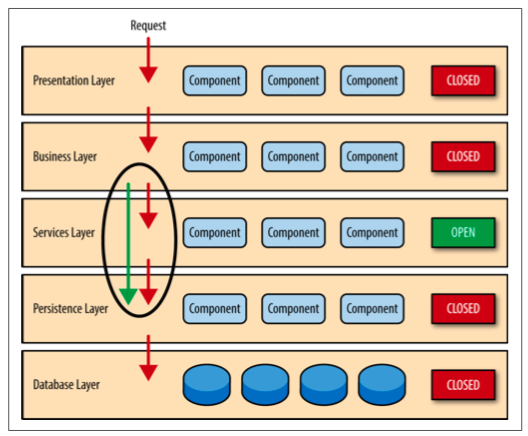
\includegraphics[width=10cm]{Monografia-FormatoLatex/Imagens/open-layer.png}
        \end{center}
    }
    \legend{Fonte: Imagem retirada do livro \citeonline[Cap.~1]{Richards2015}}.}}
    \label{fig:open-layer}
\end{figure}


\section{Hipótese}

A arquitetura baseada em Microsserviços:
\begin{itemize}
    \item Implementação arquitetural rápida
    \item Escalar a aplicação de forma fácil e com diminuição de custos
    \item Fácil manutenabilidade
    \item Fácil utilização de várias linguagens de programação
    \item Deploy rápido e fácil
    \item Logs difíceis de manter
    \item Fácil implementação de autorização e autenticação
\end{itemize}

\section{Objetivo Geral}

O objetivo do trabalho é implementar e verificar o quão complexo é implementar as arquiteturas em camadas e a baseada em microsserviços e analisar a escalabilidade, manutenibilidade, o uso de multi tecnologias, a facilidade do deploys, a verificação dos logs, implementação e manutenção da autorização e autenticação nas duas arquiteturas e fazer uma comparação empírica entre ambas.

\section{Justificativa}

Com o avanço das tecnologias os engenheiros precisam estar preparados para lidar com problemas arquiteturais complexos, haja visto a complexidade dos sistemas que estamos desenvolvendo hoje em dia. \cite{Schmidt2018} explana o quanto precisamos entender melhor sobre as arquiteturas, tanto as vantagens, quanto as desvantagens. Com o desenvolvimento dos softwares modernos e com softwares cadas vez mais distribuídos em conceitos como \textbf{cloud}, infra-estrutura e plataforma como serviço, precisamos de mais estudos científicos sobre as arquiteturas e mais especificamente a baseada em microsserviços, não é uma arquitetura nova, porém é uma evolução de modelos antigos para os sistemas de hoje.

Há inconvenientes quando se implementa uma arquitetura em camadas sem se planejar, como já dito suas vantagens e desvantagens devem ser levadas em consideração e também o projeto e equipe. \cite{Schmidt2018} propõe que os arquitetos e os engenheiros devem entender todas as características das diversas arquiteturas que já foram catalogadas. Há poucos artigos cientifico sobre arquiteturas de modo geral e também especificamente sobre a arquitetura baseada em microsserviços.

O aprendizado em arquitetura e a experiência sobre softwares mal planejados fazem com que esse trabalho seja importante para entender melhor as arquiteturas propostas nesse projeto. Esse trabalho é importante não só para a formação, mas pela identificação com essa temática da engenharia de software.


\section{Método}

Para o proposito deste trabalho será estabelecido o estudo da arquitetura de microsserviços, analisando todo o fluxo entre as partes que compõe as arquiteturas.A implementação é uma parte fundamental desse trabalho, haja visto que com as implementações feitas, poderemos obter dados empírico e também dados analíticos.

Dito o resumo acima o método utilizado será:
 \begin{itemize}
     \item Levantamento bibliográfico sobre os tópicos abordados neste trabalho como: Arquiteturas, Microsserviços, Sistemas distribuídos e outros;
     \item Pesquisar sobre a Arquitetura de Microsserviços  e sua implementação;
     \item Definição das ferramentas para a construção da arquitetura de Microsserviços;
     \item Escolha das tecnologias;
     \item Modelagem da arquitetura pensando nas ferramentas e nas vantagens da ferramenta;
     \item Implementação da arquitetura com a utilização das tecnologias Open Source;
     \item Com um navegador analisar o tempo de requisição e resposta. Relatar o esforço para a implementação de ambas as arquiteturas. Efetuar testes no desligamento do servidor e analisar como se comporta o sistemas.
     \item Testar e documentar os resultados
 \end{itemize}
     % Introdu\c{c}\~{a}o
%% TCC - Monografia
%% Ci\^{e}ncia da Computa\c{c}\~{a}o - LCMAT - CCT - UENF, 2018
%% 

% definições
% arquiteturas
% arquitetura -> camadas e monolítico
% Ruby 
% Framework Rails
% deploy
% pipeline
% protocolos
% protocolos http e http/2
% ssl e TSL
% webservice
\chapter{Arquitetura de software}\label{cap2}

A arquitetura de software de modo geral tem por objetivo apresentar a comunicação entre cada camada do sistema, bem como, suas limitações, características e interfaces como bem definido por \cite{Sizo2010}. O trabalho tem por objetivo descrever as arquiteturas baseadas em camadas e microsserviços.

% focará em duas arquiteturas bem conhecidas no momento em que essa monografia está sendo escrita, são elas a arquitetura monolítico e a de Microsserviços.
Neste capítulo serão apresentadas diversas tecnologias, conceitos e definições que compõe as duas arquiteturas. Quando tratarmos de ferramentas iremos deixar claro que o intuito não é a ferramenta utilizada, mas os conceitos utilizados por elas, entretanto, deixaremos sempre em aberto a melhor tecnologia a ser aplicada, porém vamos utilizar algumas tecnologias como Node.js (http://nodejs.org), Firebase (http://firebase.google.com) e outras para conseguirmos chegar a conclusões concretas.

\section{Arquitetura}

\subsection{Decisões de Arquitetura}

Os desenvolvedores normalmente iniciam os projetos sem um planejamento de arquitetural adequada. Quando não se pensa no projeto como um todo e se desenvolve esse novo sistema de maneira desorganizada, a aplicação poderá sofrer grandes problemas conforme for crescendo, devido a falta de padrão. Naturalmente como já descreve  \cite{Richards2015} os projetos são desenvolvidos utilizando a arquitetura em camadas ou também chamada de arquitetura monolítica. Com uma arquitetura monolítica desorganizada, teremos módulos ou classes desorganizados e muitas responsabilidades em lugares inapropriados. Os engenheiros de softwares precisam entender e sempre justificar a decisão do uso daquela arquitetura.

% Seguindo essa estrutura o que acaba se tendo é uma quantidade de módulos ou classes com código desorganizado que não possuem responsabilidade e relacionamentos definidos entre os mesmos.
% Os engenheiros precisam conhecer as arquiteturas e sempre justificar as decisões do uso, principalmente quando se trata de uma arquitetura específica, como a de microsserviços.

Engenheiros de software e programadores implementam, corrigem, melhoraram, então repetem o ciclo de desenvolvimento. Após todas essas etapas, que são feitas por diversas vezes, a equipe inicia a fase de pensar em reconhecer ou melhorar a arquitetura que atende aquele sistema. Não é um processo fácil, a busca pela identificação da arquitetura ideal leva-se tempo, mas se faz necessário partir de um ponto inicial, \cite{Richards2015} descreve bem sobre essas etapas.

\subsubsection{Arquitetura em camadas ou monolítica}

A arquitetura em camadas/monolítica organizada em camadas horizontais, cada camada tem funções específica dentro do aplicativo (por exemplo, lógica de negócio, apresentação, persistência e banco de dados). No há uma quantidade ou tipo de camadas na arquitetura monolítica, mas naturalmente utiliza-se quatro camadas, são elas: lógica de negócio, apresentação, persistência e banco de dados como dito por \cite{Richards2015} como podemos verificar na figura \ref{fig:layered-architecture} . Em algumas descrições desse tipo de arquitetura pode se encontrar também três camadas como apresentação, camada de negócio e banco de dados. Aplicações menores normalmente seguem as três camadas, porém quanto maior e mais complexo mais camadas são acrescentada.


\begin{figure}[htbp]
    \hypertarget{arquitetura-camadas3}{%
        \caption{Arquitetura em camadas}
        \begin{center}
          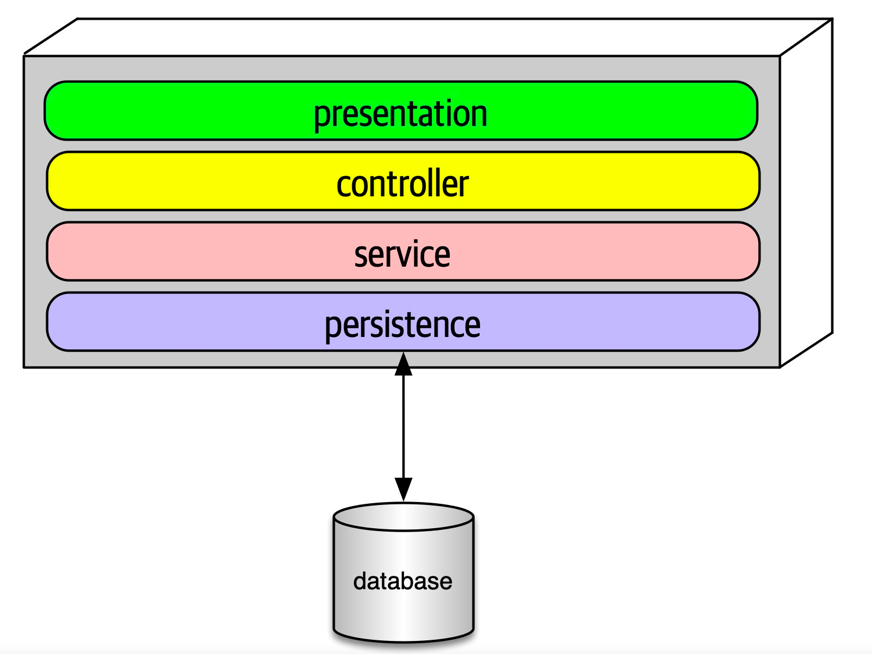
\includegraphics[width=10cm]{Monografia-FormatoLatex/Imagens/layered-architecture.png}
        \end{center}
    }
    \legend{Fonte: Imagem retirada do livro \citeonline[Cap.~4]{ford2020}}}.}}
    \label{fig:layered-architecture}
\end{figure}



As camadas na arquitetura tem função e responsabilidade específicas na aplicação. Podemos especificar algumas, como por exemplo a camada de apresentação que é responsável por lidar com toda a comunicação entre o sistema e o usuário que utiliza a aplicação, enquanto uma camada de negócios é responsável por executar regras de negócios específicas associadas à solicitação. Importante destacar que as camadas são abstrações e ela não precisa saber do sistema como um todo, ela só receber as informações que precisa para ser mostrada. Por exemplo, a camada de apresentação não precisa saber a regra de negócio, só exibir os dados para o usuário. \cite{Richards2015} explica muito bem as camadas, mas para um melhor entendimento, o cálculo é feito na camada de negócio, por exemplo 5 + 4, e a camada de apresentação só irá mostrar o valor final 9.

A arquitetura em camadas ou também conhecida como monolítica tem sido a mais utilizada por anos, haja visto que é uma das arquiteturas que mais temos conhecimento quanto a vantagens e desvantagens, pois há diversos artigos e também há uma experiência devido o tempo que trabalhamos com ela segundo \cite{Batista2018}.

A arquitetura monolítica pode ser descrita como um sistema centralizado, onde todas as responsabilidades e funcionalidades estão em um mesmo sistema, se por algum motivo um servidor pausar/falhar a aplicação inteira é afetada e nenhum usuário poderá utilizar a aplicação. Nesse tipo de arquitetura temos as algumas camadas que são elas: negócio, apresentação e dados, dependendo do modelo de arquitetura em camadas podemos ter outras como mostrado na figura \ref{fig:open-layer2}.

Podemos descrever algumas vantagens dessa tipo de arquitetura, por exemplo as camadas seguem uma hierarquia, as dependências são centralizadas, os códigos reutilizáveis e as regras de negócio também. Aplicações monolíticas são fáceis de serem desenvolvidas, afinal são ferramentas especializadas em uma única aplicação.

Como qualquer coisa específica, tem também suas desvantagens como descreve \cite{Batista2018}, a escalabilidade, agregação de novas tecnologias e a curva de aprendizado pode-se tornar alta e dependendo da regra de negócio, pode também ficar mais complexo, pois há uma grande base de código.

% \begin{figure}[htbp]
% \hypertarget{arquitetura}{%
% \caption{Arquitetura em camadas e o seu fluxo}

% \begin{center}
% 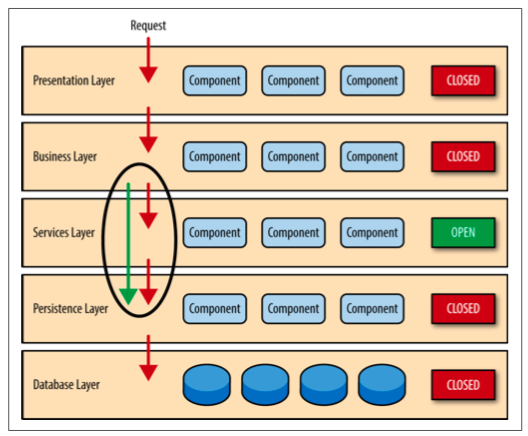
\includegraphics[width=10cm]{Monografia-FormatoLatex/Imagens/open-layer.png}
% \end{center}
% }
% \legend{Fonte: Imagem retirada do livro \citeonline[Cap.~1]{Richards2015}}.}}
% \label{mvc}
% \end{figure}


\begin{figure}[htbp]
    \hypertarget{arquitetura-camadas2}{%
        \caption{Arquitetura baseada em microsserviços}
        \begin{center}
          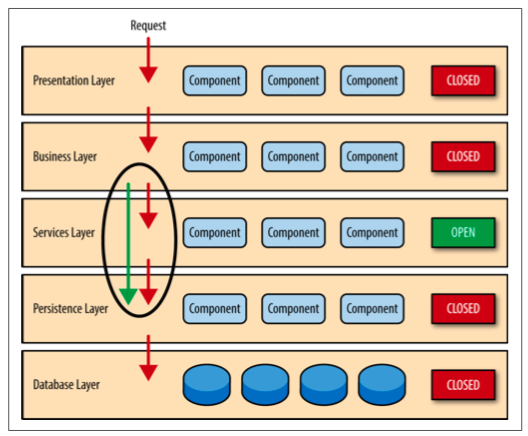
\includegraphics[width=10cm]{Monografia-FormatoLatex/Imagens/open-layer.png}
        \end{center}
    }
    \legend{Fonte: Imagem retirada do livro \citeonline[Cap.~1]{Richards2015}}.}}
    \label{fig:open-layer2}
\end{figure}



\subsubsection{Arquitetura de Microsserviços}


A arquitetura baseada em microsserviços ganhou muito destaca nos últimos anos por causa das grandes corporações que precisava escalar as suas aplicações de forma mais rápida e menos custosa e também para que suas equipem possam ter mais produtividade, haja visto que é melhor um colaborador trabalhar em um pequeno sistema, do que trabalhar com diversos sistemas complexos e que poderia gerar grandes prejuízos as empresas caso tenha alguma falha. \cite{Richards2015} explica que ainda há muitas dúvidas sobre o padrão baseado em microsserviços e a melhor forma de projetar esse tipo de arquitetura.

Buscaremos um modo para implementar esse tipo de arquitetura ao longo deste trabalho, porém é importante entender que há várias formas de se implementar a mesma arquitetura. Há conceitos que são pré requisitos para que a arquitetura seja considerada baseada em microsserviços, entretanto há formas mais elaboradas ou menos elaboradas. Cada micro serviço segue o princípio de responsabilidade única e tem como princípio que cada componente da arquitetura o isolamento desse sistema, com banco de dados próprio e comunicação via mensageria ou json por exemplo. Suas vantagens são perspetiveis em seus conceitos, onde podemos analisar brevemente que um sistema menor é mais simples de dar manutenção do que um sistema mais complexo, porém se faz necessário uma análise mais ampla as arquiteturas como \cite{Richards2015} expõe.

% Neste trabalho seguiremos um modo de implantação, porém é importante lembra-se que há várias formas de implementar, entretanto, há conceitos fundamentais para esse tipo de arquitetura. O conceito de software de responsabilidade única tem como princípio que cada componente da arquitetura de microsserviços é desenvolvida como uma unidade e há uma vantagem imediata, torna-se fácil o a entrega efetiva, construção de testes, escalabilidade e um alto grau de desacoplamento, pois a aplicação tem um contexto e esse contexto é uma aplicação pequena.

% A arquitetura baseada em microsserviços tem ganhado espaço em sistemas que necessitam escalar rapidamente como alternativa ou complemento a arquitetura em camadas ou também conhecida como monolítico. \cite{Richards2015} descreve que este tipo de arquitetura tem evoluindo, há ainda muitas dúvidas sobre esse padrão e no como implementar.
% Neste trabalho seguiremos um modo de implantação, porém é importante lembra-se que há várias formas de implementar, entretanto, há conceitos fundamentais para esse tipo de arquitetura. O conceito de software de responsabilidade única tem como princípio que cada componente da arquitetura de microsserviços é desenvolvida como uma unidade e há uma vantagem imediata, torna-se fácil o a entrega efetiva, construção de testes, escalabilidade e um alto grau de desacoplamento, pois a aplicação tem um contexto e esse contexto é uma aplicação pequena.

Com essa arquitetura necessitamos modificar a forma como desenvolvemos software de modo geral, como por exemplo pensar em componentes de serviços, no caso desse tipo de arquitetura a cada componente serviço pensado, teremos um sistema. A arquitetura pode conter um ou mais módulos ( por exemplo, classes em Ruby ou funções em Elixir) que representam um contexto de negócio único ( por exemplo, fornecer boletos para o usuário) ou mais ainda um aplicativo de negócios de grande porte (por exemplo, financeiro de uma empresa). \cite{Richards2015} explica que projetar o nível de granularidade dos componentes de serviço é um dos maiores desafios dos microsserviços.
% É importante pensar em componentes de serviços, que pode variar de um único módulo a uma grande parte do aplicativo. A arquitetura pode conter um ou mais módulos ( por exemplo, classes em Ruby ou funções em Elixir) que representam um contexto de negócio único ( por exemplo, fornecer boletos para o usuário) ou mais ainda um aplicativo de negócios de grande porte (por exemplo, financeiro de uma empresa). \cite{Richards2015} explica que projetar o nível de granularidade dos componentes de serviço é um dos maiores desafios de uma arquitetura de microsserviços.

Alguns conceitos chaves descritos por \cite{Richards2015} necessitam serem compreendidos, por exemplo os conceitos de sistema distribuídos. A arquitetura baseada em microsserviços segue os conceitos de sistemas distribuídos como já dito, isso significa que todos os componentes da arquitetura são desacoplados e acessados por meio de algum tipo de comunicação de acesso (por exemplo, AMQP, REST, SOAP, RMI, etc). É por isso que ela alcança as características de escalabilidade e implantação de forma superior a outras arquiteturas.

% É importante entender que essa arquitetura segue alguns conceitos chaves que \cite{Richards2015} cita, como ele é uma arquitetura com sistemas distribuídos, isso significa que todos os componentes da arquitetura são dissociados e acessados por meio de algum tipo de protocolo de acesso remoto (por exemplo, AMQP, REST, SOAP, RMI, etc). É por isso que ela alcança as características de escalabilidade e implantação de forma superior a outras arquiteturas.

Como já dito acima, não é pré-requisito a utilização de todos os componentens para se ter uma arquitetura baseada em microsserviços, porém para esse trabalho iremos utilizar um microserviço chamado API Gateway. O \cite{Florez2016} explica o quão benéfico é ter a API Gateway para lidar com diferentes solicitações de API, roteando-as para os microsserviços apropriados. Se você usa o API Gateway, projete e implemente-o com cuidado para evitar o acoplamento entre serviços. Cada microsserviço pode ter vários microcomponentes que podem ser separados em diferentes camadas. A \ref{fig:microsserviços} mostra esse tipo de microsserviço.

% \begin{figure}[htbp]
% \hypertarget{arquitetura}{%
% \caption{Arquitetura baseada em microsserviços}
% \label{microsserviços}
% \begin{center}
% 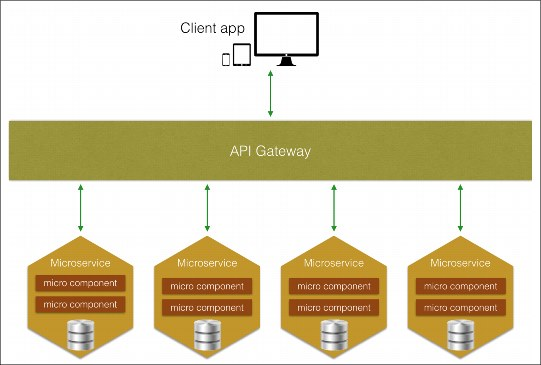
\includegraphics{Monografia-FormatoLatex/Imagens/api-gateway.jpg}
% \end{center}
% }
% \legend{Fonte: Imagem retirada do livro \citeonline[Cap.~2]{Florez2016}}.}}
% \end


\begin{figure}[htbp]
    \hypertarget{arquitetura-microservice1}{%
        \caption{Arquitetura baseada em microsserviços}
        \begin{center}
          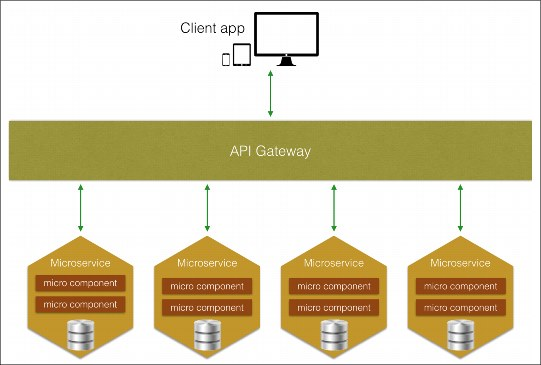
\includegraphics[width=10cm]{Monografia-FormatoLatex/Imagens/api-gateway.jpg}
        \end{center}
    }
    \legend{Fonte: Imagem retirada do livro \citeonline[Cap.~2]{Florez2016}}.}}
    \label{fig:microsserviços}
\end{figure}


 Sistemas baseados puramente na arquitetura de microsserviços seguem algumas características que \cite{TomasCerny2017} explora em seu artigo, são elas:
 
 \begin{itemize}
   \item O programa deve ter uma só tarefa e executar bem. Exemplo: gerador de PDF, ele só vai gerar PDF e fará muito bem essa função.
   \item A aplicação deve ser fácil de ser integrada a outros softwares. Qualquer aplicação que queira gerar PDF, poderá gerar facilmente.
   \item O gerador de PDF deve utilizar uma interface única com os outros sistemas, tudo de forma transparente para o usuário ou sistemas que irão utilizar.
 \end{itemize}

O \cite{Batista2018} define a arquitetura de Microsserviços como uma estrutura descentralizada, onde todas as camadas da aplicação ficam em servidores próprios e ambos se comunicam através das APIs. A forma de comunicação torna-os totalmente independentes e autônomos.

Uma descrição interessante é a dos autores do artigo \cite{Zhu2016} onde eles definem os microsserviços como sistemas que cada serviço é pequeno (daí o "micro") e que todos os desenvolvedores desses serviços entendam que estão trabalhando no mesmo sistema.

Esse tipo de arquitetura tem diversas vantagens como \cite{Batista2018} cita: 

\begin{itemize}
    \item Utiliza-se de comunicação leve e simples atráves do protocolo HTTP e com o HTTP version 2 a comunicação se tornou mais rápida.
    \item A utilização de qualquer linguagem de programação que o desenvolvedor queira utilizar.
    \item Permite experimentar e testar
    \item Bancos de dados diferentes
\end{itemize}

Com esse tipo de arquitetura há um ganho na diminuição de falhas, haja visto que são independentes, caso um sistema de pagamentos caia, o gerador de boletos, por exemplo continua funcionando. 
Entretanto esses benefícios não param por aí, como diz \cite{Tom2016} há diversos benefícios escondidos, ele dá alguns tópicos como: Inovação sem permissão, permissão para falhar, Interromper com confiança, você constrói, você mantém, acelera as descontinuações, testa de forma diferente, finaliza metadados centralizados, concentra a dor, caso tenha se interessado e deseja mais informações é sugerido que leia o artigo completo.

Uma das desvantagens que devemos nos preocupar quando estamos utilizando esse tipo de arquitetura é no contexto específico da aplicação e a complexidade entre a comunicação dos sistemas.


\subsection{ REST API}

REST significa REpresentational State Transfer, que é um estilo de arquitetura, e não um protocolo como definido muito bem no artigo \cite{Harber2019}.

\cite{Harber2019} descreve que a API é uma abreviação de interface de programa de aplicativo, que permite que os aplicativos se comuniquem. No caso da web, uma API é normalmente um conjunto de URLs que respondem com dados quando chamados da maneira correta e com as informações corretas.

Uma API REST é uma interface sem estado para seu aplicativo. No caso da pilha MEAN (Mongo, Express, Angular e NodeJS), a API REST é usada para criar uma interface sem estado para seu banco de dados, permitindo que outros aplicativos, como um SPA Angular, trabalhem com os dados. Em outras palavras, você cria uma coleção de URLs estruturadas que retornam dados específicos quando chamados, essa definição também é descrita por \cite{Harber2019}.


\subsection{Computação em nuvem}

A Computação em nuvem de forma simplista é levar ao usuário final, seja ele empresas ou pessoas físicas uma infraestrutura, plataforma ou software complexo, através de serviços simples e acessível de qualquer computador com um navegador instalado. Como \cite{Sousa2010} referencia no seu artigo, computação em nuvem é uma tendencia para os dias atuais e tem o objetivo entregar serviços sobre demanda, com pagamento baseado na utilização. Caso se interesse no assunto, o artigo do \cite{Sousa2010} é interessante para se aprofundar nesse conceito.

\cite{Hanjura2014} descreve que os serviços oferecidos pela computação em nuvem são divididos em diferentes modelos de serviço - infraestrutura como serviço (IaaS), plataforma como serviço (PaaS) e software como serviço (SaaS) como podemos verificar na figura \ref{fig:arquitetura-nuvem} . Essa classificação é feita para separar os diferentes tipos de serviços que um usuário pode adquirir para atender às necessidades de negócios em um ambiente de computação em nuvem.


% \begin{figure}[htbp]
% \hypertarget{arquitetura}{%
% \caption{ Alguns serviços suportados pela computação em nuvem }
% \label{fig:arquitetura-nuvem}
% \begin{center}
% 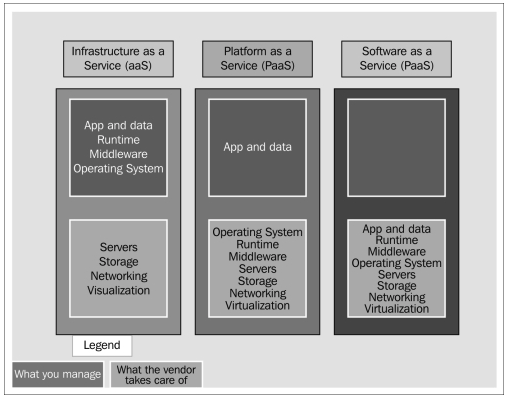
\includegraphics{Monografia-FormatoLatex/Imagens/computacao_em_nuvem.png}
% \end{center}
% }
% \legend{Fonte: Imagem retirada do livro \citeonline[Cap.~1]{Hanjura2014}}}.}}
% \end


\begin{figure}[htbp]
    \hypertarget{arquitetura-nuvem}{%
        \caption{Alguns serviços suportados pela computação em nuvem}
        \begin{center}
          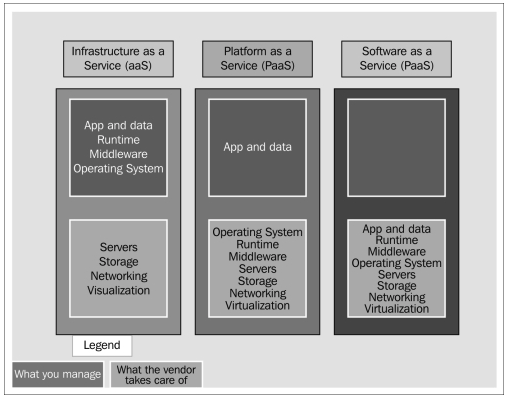
\includegraphics[width=10cm]{Monografia-FormatoLatex/Imagens/computacao_em_nuvem.png}
        \end{center}
    }
    \legend{Fonte: Imagem retirada do livro \citeonline[Cap.~1]{Hanjura2014}}.}}
    \label{fig:arquitetura-nuvem}
\end{figure}

A nuvem é classificada em alguns modelos de serviços. Cada modelo fornece um serviço distinto. Os modelos são IaSS, BaSS, PaSS e SaSS. Como \cite{Evangelista2016} cita em seu artigo a sigla em inglês significa Infrastructure as a Service (IaaS), Backend as a Service,  Plataform as a Service (PaaS) e Software as a Service (SaaS).

\subsection{Infrastructure as a Service (IaaS)}

É o tipo de modelo de serviço que permite ao usuário final utilizar capacidade de processamento, redes de dados, memória ram, SSD, sistema operacional e diversos componentes de hardware e rede. O IaSS permite gerenciar todos os recursos através de interfaces gráficas. Exemplo de IaSS: AWS, Google Cloud e Digital Ocean.

A definição de IaaS feita por \cite{Hanjura2014} é que o modelo de serviço em nuvem que permite ao usuário fornecer recursos de hardware virtualizado sob demanda. Fisicamente, esses recursos podem se espalhar por vários data centers, mantidos pelo provedor de serviços. Esses recursos incluem armazenamento virtual, conexões de rede e balanceadores de carga para o recurso de hardware provisionado. O usuário pode usar o recurso sob demanda e pagar por uso. Se o usuário precisar de mais recursos, o provedor poderá escalar automaticamente o hardware de acordo com a necessidade e vice-versa. Um bom exemplo de um provedor de IaaS é o Amazon Web Services (AWS - http: //aws.amazon.com). É o provedor de IaaS mais popular na nuvem. Rackspace (http://www.rackspace.com) é outro exemplo.


\subsection{Plataform as a Service (PaaS)}

É o modelo de serviço que levanta um servidor de diversas linguagens sem muito esforço. O usuário não tem acesso a infraestrutura, rede, dependências do sistema operacional e não precisa se preocupar com a atualização da mesma. Contrata só as configurações da plataforma.

A definição de PaaS feita por \cite{Hanjura2014} é que o modelo de serviço em nuvem que fornece as ferramentas para criar aplicativos de software na nuvem. Uma analogia próxima seria considerar o PaaS como um sistema operacional e um middleware do ambiente em nuvem. O PaaS fornece aos desenvolvedores a plataforma subjacente a ser usada para desenvolver seus aplicativos. Ele cuida do suporte a um idioma ou tecnologia específica que os desenvolvedores da pilha desejam usar. Muitos provedores de PaaS também permitem o dimensionamento sob demanda dos recursos subjacentes de computador e armazenamento, automaticamente, para liberar o usuário da nuvem da tarefa de alocar recursos manualmente. No PaaS, o consumidor do serviço controla a implantação e a configuração. O provedor PaaS provisiona os servidores, a rede e as necessidades computacionais do aplicativo de software. O modelo PaaS também permite uma arquitetura multitenant (definir isso) para que vários usuários possam usar o aplicativo da Web de maneira segura, escalável, simultânea e à prova de falhas. As sofisticadas soluções PaaS também fornecem um ambiente integrado de desenvolvimento de aplicativos da web, o que facilita a codificação colaborativa, o controle da fonte e a implantação. Heroku (http://www.heroku.com) e Google App Engine (http://cloud.google.com/AppEngine) são dois exemplos de plataformas PaaS de sucesso.

\cite{Hanjura2014} descreve que embora o PaaS seja inerentemente mais estável em comparação com o componente SaaS. PaaS evoluiu enormemente nos últimos anos e forneceu à comunidade de desenvolvedores ferramentas incríveis (menos adjetivo!) para trabalhar e implantar aplicativos distribuídos praticamente em pouco tempo.

\subsubsection{Heroku}

\cite{Hanjura2014} descreve o Heroku (http://www.heroku.com) como um dos principais fornecedores de PaaS no negócio de software em nuvem, provando ser a solução PaaS líder em pequenas e grandes empresas. Com melhorias consistentes e a filosofia de "conveniência" sobre "configuração", o Heroku se tornou a principal plataforma de desenvolvimento de aplicativos em nuvem para desenvolvedores. A filosofia da Heroku é permitir que os desenvolvedores se concentrem apenas em escrever aplicativos da Web e esquecer os servidores. O Heroku cuida magicamente da criação, implantação, execução e dimensionamento do aplicativo para o desenvolvedor sob demanda.


\cite{Hanjura2014} descreve o Heroku como uma plataforma de aplicativos em nuvem poliglota que oferece uma enorme flexibilidade na escolha de uma linguagem de programação apropriada para o desenvolvimento de aplicativos da web. O Heroku fornece suporte de plataforma para Ruby, Ruby on Rails, Java, Node.js, Clojure, Scala, Python e PHP a partir do início de 2013.

\subsection{Software as a Service (SaaS)}
É o modelo em que o usuário tem a aplicação disponível em tempo real através dos smartfones ou dos navegadores. O usuário não tem acesso a infraestrutura ou a plataforma, tudo é transparente para o usuário através de uma interface simples. O usuário só poderá configurar aspectos restritos da própria aplicação.

A definição de SaaS feita por \cite{Hanjura2014} é que o modelo SaaS da nuvem fornece software que você pode consumir do alcance do seu navegador da web. Não há necessidade de instalações complexas e demoradas. Abra um navegador, aponte para um URL e use o aplicativo apontado pelo URL. O que acontece nos bastidores está oculto ao usuário. O SaaS evoluiu consideravelmente na última década. Muitos provedores de SaaS tornaram obsoleto o software para desktop ou hospedado localmente. Tudo que você precisa é de um navegador e está pronto para usar qualquer aplicativo para fazer qualquer coisa. Sem dores de cabeça de atualizações de software, incompatibilidade de versão ou portabilidade de software. O serviço Gmail (http://gmail.com) do Google é uma das implementações de SaaS mais bem-sucedidas e conhecidas. O componente SaaS cresceu exponencialmente com empresas aproveitando a infraestrutura e a plataforma subjacentes para criar versões em nuvem da maioria de suas ofertas de produtos de software. Em 2013, quase todas as empresas que valem a pena ter uma versão SaaS de seus aplicativos populares de software disponíveis para clientes on-line.


\subsection{DevOps}

O DevOps é um conjunto de práticas ou uma cultura com o propósito de diminuir o tempo entre uma mudança feita e submetida em produção de forma a garantir a qualidade, seja em código ou seja em testes. O autor ainda descreve que toda mudança gera impactos nos processos, produtos, tecnologias utilizadas e estrutura organizacional, haja visto que estamos lidando com uma nova abordagem. A implantação dessa cultura não é fácil, muitas das vezes haverá tensões na organização e no negócio, pois terá que ser modificada a forma de trabalho diário como descreve \cite{Zhu2016}.

\cite{Zhu2016} descreve sobre os efeitos que o DevOps têm sobre os desenvolvedores ao longo do processo de desenvolvimento de software, ele lista alguns itens que valem a pena serem citados. São eles: 

\begin{itemize}
    \item Integração contínua é uma prática que deve ser utilizada e ela é o ato de submeter um código para um repositório central e o software executar os testes automatizados e subir para homologação ou produção sem que haja uma pessoa que cuide desse processo.
    \item Os sistemas são monitorados e após uma implementação, caso o haja alguma falha é possível reverter as alterações.
\end{itemize}

A utilização dessa cultura depende muito de diversas ferramentas, são elas: gerenciamento de contêineres, integração contínua, orquestração, monitoramento, implantação e teste. O \cite{Zhu2016} cita que cada vez mais, os engenheiros de software mantêm e configuram essas ferramentas.


\subsubsection{Docker}

Docker é uma aplicação que virtualiza os servidores, essa ferramenta foi desenvolvida para fornecer, via receita, um ambiente de forma rápida, seja para desenvolvimento ou produção. Todas às vezes ao inicializar um servidor necessitamos de um processo manual que se repete diversas vezes e que podemos automatizar e o docker torna esse processo simples. 

O Docker é considerada uma plataforma de virtualização em containers, ajuda os desenvolvedores a inicializar o ambiente sem esforço, basta ter a plataforma instalada localmente e conseguirá desfrutar dos benefícios de instalar sua aplicação, sem a necessidade de utilizar os arquivos da sua máquina física, em pouco minutos através do build da plataforma terá um ambiente totalmente configurado. O docker é uma tecnologia de código aberto, como \cite{Ouverney2017} descreve em seu artigo, durante o build é criado um container com todas dependências instaladas e a aplicação pronta para uso. Essa plataforma ajuda na implementação da arquitetura de microsserviços, pois cada aplicação fica isolada em um container, não afetando o funcionamento dos outros serviços.

\subsubsection{Testes automatizados}
 Durante o desenvolvimento de uma determinado sistema nos deparamos com diversos cenários de repetição de tarefas e, quando uma tarefa é repetitiva e pode ser automatizada, podemos automatizar esse processo, o que nos permite focar na resolução do problema que desejamos resolver. Os computadores fazem tarefas repetitivas melhor do que os humanos, o \cite{Bernardo2008} descreve em seu artigo, precisamos pensar em qualidade e nas inúmeras dificuldades quando se trata de questões humanas, então, porque não automatizar os testes, pois há processos repetidos que faríamos e poderemos falhar por falta de atenção em um dado momento.

A cultura DevOps já define em seus processos a automatização dos testes de software, \cite{Bernardo2008} define que os testes automatizados é uma técnica voltada a qualidade de software, onde uma alteração que possa quebrar o sistema, facilmente será percebida pelos desenvolvedores em poucos minutos. Existem alguns exemplos de testes, mas não se torna necessário descrever cada um deles, caso sinta-se curioso para saber mais sobre o artigo do \cite{Bernardo2008} lhe trará uma visão mais ampla sobre os tipos de teste.


\section{Tecnologias}

Nessa seção abordaremos algumas tecnologias e empresas que hospedam essas tecnologias para utilizarmos no dia a dia e de forma colaborativa.

\subsection{Git}

\cite{Beer2018} explica que o Git é um sistema de controle de versão. Esse tipo de software é projetado para acompanhar as alterações feitas nos arquivos ao longo do tempo. Ele explica ainda que o git é um sistema de controle de versão distribuído, o que significa que todos os que trabalham com um projeto no Git tem uma cópia do histórico completo do projeto, não apenas do estado atual dos arquivos.

\subsubsection{Github}

O Github é uma plataforma onde se pode fazer upload de uma cópia do seu repositório Git e de forma fácil toda sua equipe poderá fazer um clone do projeto e trabalhar simultaneamente no mesmo projeto como dito por \cite{Beer2018}. Ele ainda explica que o Github faz isso fornecendo um local centralizado para compartilhar o repositório, uma interface baseada na Web para visualizá-lo e recursos como fork, pull request, wiki do Github que permite especificar, discutir e revisar alterações com a sua equipe de forma mais eficaz. Caso queira saber mais informações basta acessar o site http://github.com.

\susubsection{Gitlab}

O Gitlab é uma plataforma de código aberto para armazenar uma cópia do seu repositório git, igualmente ao Github, podemos ter mais informações sobre o mesmo no \cite{Baarsen2014} ou no próprio site http://gitlab.com.

\subsection{Linguagem de Programação e Framework}

\subsubsection{ Node.js }

\cite{Herron2018} descreve o Node.js como uma nova e empolgante plataforma para desenvolvimento de aplicativos web e servidores de aplicativos. Essa tecnologia é detalhada como um projeto que trás extrema escalabilidade em aplicativos e em rede através de uma combinação engenhosa de JavaScript do lado servidor, I/O assíncrona e programação assíncrona. Ele é construído em torno de funções anônimas JavaScript e uma arquitetura orientada a eventos de encadeamento de execução única.

\cite{Herron2018} nos da uma informação importante sobre threads, o Node.js evita os threads por causa de sua complexidade. É dito que, com arquiteturas orientadas a eventos de thread única, o espaço ocupado na memória é baixo, o rendimento é alto, o perfil de latência de carga é melhor e o modelo de programação é mais simples. A plataforma Node.js está em uma fase de rápido crescimento, e muitos a veem como uma alternativa atraente às arquiteturas de aplicativos da web tradicionais usando Java, PHP, Python ou Ruby on Rails.

\subsubsection{React Native}

 React Native é uma estrutura de desenvolvimento de aplicativos na qual você usa tecnologias padrão da Web (ou, em alguns casos, algo semelhante às tecnologias padrão da Web) para criar seu aplicativo. Isso significa algo parecido com o HTML, JavaScript e CSS. O React Native é baseado na estrutura React do Facebook, uma estrutura popular de desenvolvimento da web. A diferença crítica entre os dois é que o React tem como alvo os navegadores da Web, enquanto o React Native tem como alvo os smartphones e seus sistemas operacionais como descrito por \cite{Zammetti2018}.

\subsection{Banco de dados}

\subsubsection{ MongoDB }

MongoDB é um banco de dados NoSQL para a Web moderna. NoSQL significa Not only SQL, é um termo cunhado por Carlo Strozzi em 1998, por seu banco de dados de código aberto que não seguia o padrão SQL, mas ainda era relacional, segundo \cite{Giamas2019}. Caso queira se aprofundar mais sobre o MongoDB, o mesmo conta com uma documentação completa no link https://docs.mongodb.com/manual/.

\subsubsection{ PostgreSQL }

\cite{Volkov2017} descreve o PostgreSQL como um sistema de gerenciamento de banco de dados relacional de objeto de código aberto. É executado nos sistemas operacionais mais modernos, incluindo Windows, MacOS e Linux. Está em conformidade com o SQL.

\subsection{Firebase}

O \cite{Yahiaoui2017} descreve o firebase como um BaaS, um back-end como serviço, com ele evitamos instalações e configurações que não iria agregar na solução do nosso problema para o momento.

O \cite{Yahiaoui2017} cita ainda que o Firebase é um BaaS com muitos recursos que facilita a criação dos projetos e elimina muitas tarefas tediosas e já fornecendo uma plataforma segura e bem construída que nos da simplicidade e escalabilidade de forma rápida.

\subsection{Firebase Realtime Database}


\cite{Yahiaoui2017} cita que o Firebase Realtime Database é o produto mais usado pelos desenvolvedores em toda a pilha de produtos disponíveis no Firebase. Ele oferece diversas funções como atualizações, inserções e exclusões de dados em tempo real.

\cite{Yahiaoui2017} detalha que a funcionalidade de transmissão integrada e uma API extremamente simples de usar torna o Realtime Database um recurso atraente. O interessante a se destaca que a APIs oferecem aos desenvolvedores a oportunidade de explorar as APIs em uma escala maior, independentemente do ecossistema e ambiente que eles estão usando. Além disso, o Firebase Realtime Database vem com suporte offline. Esse recurso entra em ação quando o aplicativo está em um estado de rede não tão confiável.


\subsection{Firebase Authentication}

Essa funcionalidade é uma das partes centrais de qualquer sistema e o \cite{Yahiaoui2017} descreve que a criação de um sistema de autenticação seguro acaba sendo um trabalho muito tedioso, mesmo que seja apenas e-mails e senhas.

Os aplicativos tendem a utilizar login com as redes sociais também e é um dos recurso mais utilizados e solicitados no cenário atual. É uma maneira rápida de fazer com que o usuário acesse o sistema como é descrito por \cite{Yahiaoui2017}.

\cite{Yahiaoui2017} descreve que o Firebase fornece métodos de autenticação múltipla, por exemplo email e senha, login social com as principais fornecedores Google, Facebook e etc.

\section{Trabalhos relacionados}

Nesta seção são mostrados alguns trabalhos relacionados sobre arquiteturas. Os trabalhos ajudaram na elaboração desse trabalho.

O autor \cite{Moreira2015} destaca as vantagens dos microsserviços e desvantagens dessa arquitetura, mostra na prática como criar uma arquitetura de microsserviço com Java Spring Boot. De modo geral o autor destaca que há diversas arquiteturas e a de microsserviços se encaixa em contextos específicos.

O artigo \cite{Chiaradia2018} aborda conceitos das áreas de gestão de relacionamento com o cliente, CRM Social e Web 2.0, enumerando as características e os benefícios. É proposta uma arquitetura de microsserviços para o sistema de CRM Social na qual o autor apresenta os fluxos de comunicação e se propõe a criação de um modelo para servir de base para futuras implementações. 

O objetivo do artigo \cite{TomasCerny2017} é conceituar as arquiteturas SOA (Service Oriented Architecture) quanto Microsserviços e mostrar as funcionalidades de cada arquitetura. O autor analisa a arquitetura quanto a performance, complexidade, tanto de implementação, quanto a uso nos dias atuais. 

Como \cite{Pahl2016} em seu artigo com o estudo de mapeamento dos métodos, técnicas e melhores práticas em arquitetura, com uma atenção particular à aplicação na nuvem. A revisão revela que a Microsserviços ainda está em um estágio formativo. É necessária uma avaliação mais experimental e empírica dos benefícios. Este estudo também demonstrou que a automatização e facilidade da arquitetura de Microsserviços em um cloud se torna necessário para extrair as vantagens que ela pode proporcionar.

O artigo \cite{Tom2016} descreve os diversos benefícios escondidos que a arquitetura de Microsserviço proporciona aos adeptos, no caso do artigo as empresas. Há algumas vantagens que não são claras no dia a dia, entretanto o artigo esclarece 8 pontos importantes que os administradores de modo geral poderão visualizar.

A arquitetura de Microsserviços  precisa ser monitorada, devido os micro sistemas estarem totalmente desacoplados, é necessário centralizar todas as informações e aí que o artigo \cite{Ghirotti2018} nos ajuda a entender a importância dessa arquitetura.

O artigo \cite{Raji2015} é importante, devido o mapeamento de visualização na área científica com a utilização da arquitetura de micro serviços, utilizando todos os conceitos da web 2.0. Um exemplo desse uso, em que o artigo retrata e o aumento da mobilidade, onde o mesmo pode ser utilizando em qualquer dispositivo e independente do sistema operacional, atingindo um público mais amplo e buscando ter um ecossistema mais rico, criando ferramentas e sites interativos. 

% \section{Análise das abordagens}

% Utilizando todos os artigos já listados até o momento e com a ideia de unir as duas arquiteturas analisamos que podemos unir ferramentas, arquitetura e o aprendizado.

% As ferramentas tem um papel importante, pois elas são o meio de torna a arquitetura viável. Nos diversos artigos lidos, algumas ferramentas são unanimes até o momento em que este trabalho está sendo escrito, mas o intuito não é prender a teoria das arquiteturas a ferramentas, mas sim a conceitos independentes delas, pois dado momento uma outra ferramenta, pode se tornar mais eficiente e mesmo assim os conceitos ainda continuaram sendo válidos.

% A arquitetura como tema central desse trabalho permite desenvolver software de qualidade em empresas. Os artigos se relacionam normalmente a contextos de negócios e não aos serviços públicos, o trabalho busca analisar os artigos e adaptar a realidade dos serviços públicos no Brasil.

% O trabalho deseja abordar também o aprendizado durante a criação de novas funcionalidades a projetos já existentes e o artigo \cite{Souza2009} explicita sobre o processo de aprender e as dificuldades que os alunos normalmente tem ao aprender uma linguagem de programação. Com a arquitetura que será conceituada, abordaremos também sobre a diminuição dessas dificuldades com a arquitetura que será proposta nos próximos capítulos.

% O autor \cite{Barker2017} nos disponibiliza diversas formas para metrificar a performance do nosso sistema, porém para esse trabalho o navegador será a nossa ferramenta principal. Os navegadores modernos nos disponibilizam um conjunto de ferramentas chamada de Dev Tools, como base faremos toda nossa analize com o dev tools do chrome.

% \section{Web Browser Developer Tools}

% Os navegadores web mais atuais incluem diversas ferramentas para os desenvolvedores web. Essas ferramentas são chamadas de Web Browser Developer Tools e navegadores como Chrome, Firefox, Safari, Edge ou Opera disponibilizam. Ferramentas que auxilia a identificar o fluxo das requisições e respostas, prioridades, dependências, o tempo e entender o Server Push. Nesse trabalho utilizaremos o \textbf{Chrome Developer Tools}.

% \subsection{Chrome Developer Tools}

% Nos últimos anos, o navegador Chrome ganhou adoção entre os desenvolvedores, em parte devido à crescente funcionalidades de suas ferramentas para desenvolvedores Web. Estar familiarizado com os recursos pode fornecer muitas vantagens para identificar diversos problemas técnicos como descreve \cite{Ludin2017}. Para acessar a ferramenta basta seguir os seguintes passos: Abra a ferramenta de desenvolvedor escolhendo Exibir -> Desenvolvedor -> Ferramentas de desenvolvimento no menu Chrome.

% Utilizaremos a aba Network para identificarmos todos os recursos que são carregados e o seu tempo para analisarmos o tempo de resposta das arquiteturas. A aba também nos proverá informações quando inserirmos um error que pare uma parte do sistema para identificarmos se o sistema continuará a responder a outra requisições. Como podemos visualizar na imagem \ref{fig:dev-tools} há uma aba chamada de Waterfall onde podemos analisar quais recursos foram carregados e em que ordem ocorreu.

% \begin{figure}[h]
%     \centering
%     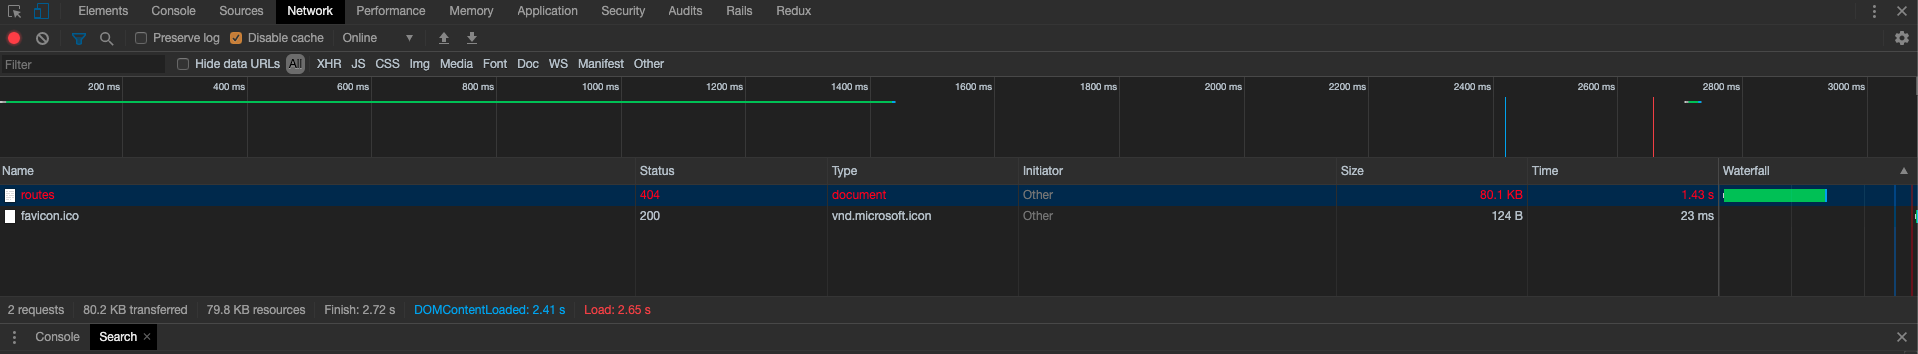
\includegraphics[width=12cm]{dev-tools.png}
%     \caption{ Imagens da aba Dev Tools do Chrome }
%     \label{fig:dev-tools}
% \end{figure}{}

% Há possibilidade de extrair diversos dados para a analisarmos como medida comparativa entre as arquiteturas, iremos utilizar a quantidade de requests feita por cada arquitetura, tamanhos dos dados transferidos, recursos recebidos e o tempo de finalização da página, esses dados serão extraídos no rodapé da ferramenta, como podemos observar na imagem \ref{fig:dev-tools2}

% \begin{figure}[h]
%     \centering
%     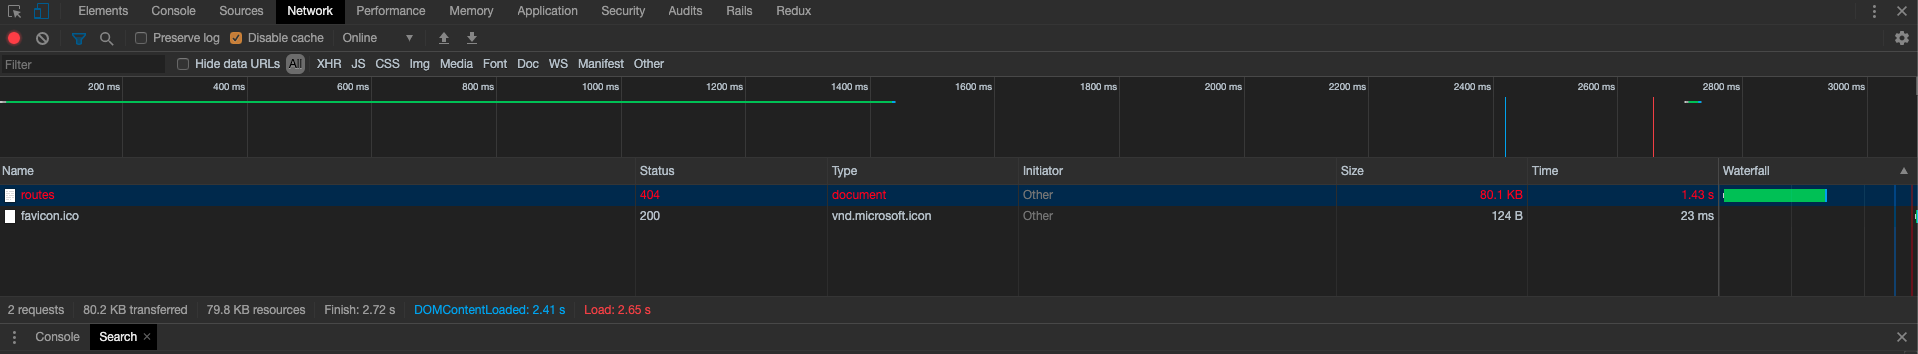
\includegraphics[width=12cm]{dev-tools.png}
%     \caption{ Imagens da aba Dev Tools do Chrome }
%     \label{fig:dev-tools2}
% \end{figure}{}        % Engenharia de
%% TCC - Monografia
%% Ci\^{e}ncia da Computa\c{c}\~{a}o - LCMAT - CCT - UENF, 2018
%% 

\chapter{Metodologia}\label{cap3}

O propósito deste trabalho é realizar um estudo descritivo sobre as arquiteturas em camadas e microsserviços. A abordagem da pesquisa será qualitativa de caráter exploratório, pois iremos focar no caráter subjetivo do objeto analisado. 

O método que será utilizado para a realização deste trabalho é o qualitativo, com a finalidade de implementar e analisar as arquiteturas, assim poderemos fazer um estudo descritivo sobre as duas arquiteturas ilustradas nesta pesquisa. Em relação ao caráter exploratório serão aplicados alguns problemas na arquitetura e analisaremos o seu comportamento.

Serão obtidos os dados necessários para essa pesquisa através das pesquisas bibliográficas, da implementação e da observação comportamental do software diante de alguns problemas que serão colocados em um ambiente controlado. Com toda essa abordagem, poderemos descrever os resultados obtidos.

A pesquisa seguirá algumas fases, que serão resumidas na sequência: 
\begin{enumerate}
    \item Revisão bibliográfica
    \item Criação do fluxo das duas arquiteturas estudadas.
    \item Implementação da arquitetura em camadas:
    \begin{itemize}
        \item Coleta de dados durante a implementação
        \item Realização de experimentos
        \item Recuperação de informação
    \end{itemize}
    
    \item  Implementação da arquitetura baseada em microsserviços:
        \begin{itemize}
        \item Coleta de dados durante a implementação
        \item Realização de experimentos
        \item Recuperação de informação
    \end{itemize}
    \item Conclusão das informações em relação à: 
    \begin{itemize}
        \item Escalabilidade, 
        \item Manutenibilidade, 
        \item Implementação computacional, assim como
        \item Vantagens e Desvantagens.
    \end{itemize}
    
\end{enumerate}

Na Figura \ref{fig:flow-metodologia} é possível observar o fluxograma da metodologia que acabamos de apresentar e que faz parte deste trabalho de pesquisa.

\begin{figure}[htbp]
    \hypertarget{arquitetura-camadas2}{%
        \caption{ Fluxograma da metodologia utilizada neste trabalho}
        \begin{center}
          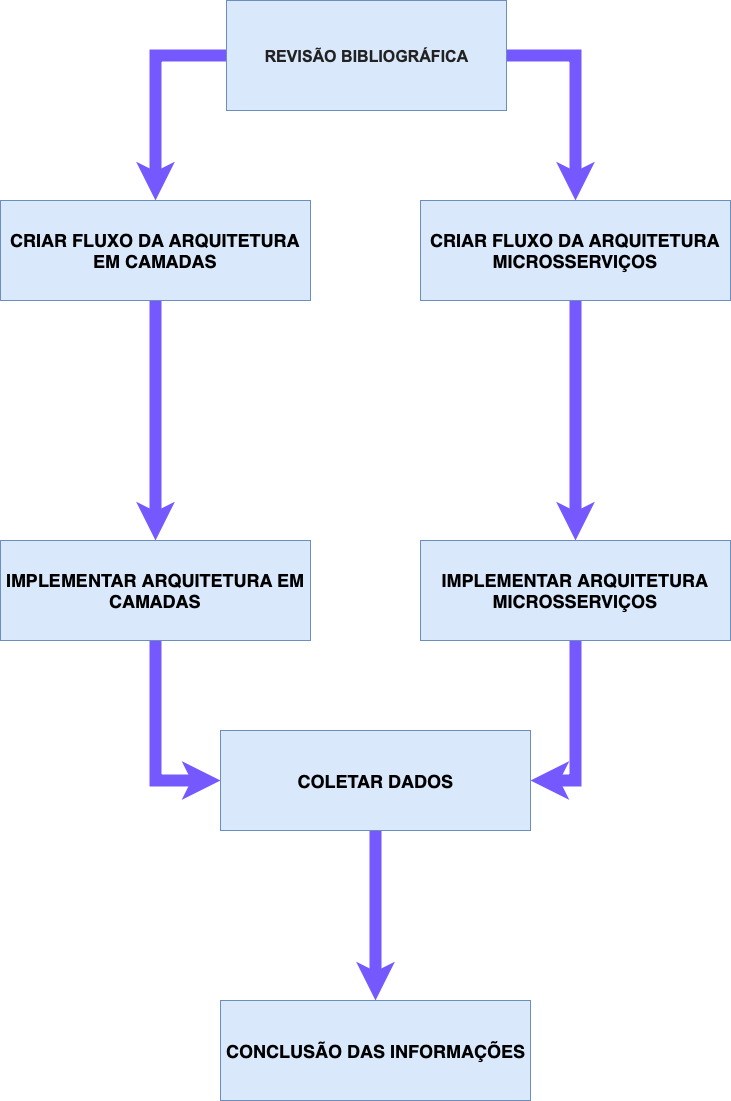
\includegraphics[width=10cm]{Monografia-FormatoLatex/Imagens/flow-metodologia.png}
        \end{center}
    }
    \legend{Fonte: Imagem feita pelo autor no site \url{draw.io}}
    \label{fig:flow-metodologia}
\end{figure}

\section{Revisão bibliográfica}
Durante essa fase, realizada no capítulo \ref{cap2}, a pesquisa buscou reunir as definições de diversos autores sobre as arquiteturas, tanto a baseada em camadas, quanto a baseada em microsserviços. Durante essa fase é importante entender o fluxo comportamental de ambas, abordagens relacionadas, informações sobre sistemas distribuídos. De modo geral nessa fase o mais importante é entender sobre as arquiteturas e porque utilizar uma ou outra.

\section{Fase 2 - Criação do fluxo das arquiteturas }

É importante durante a criação de um fluxograma para buscar a melhor tecnologias para esse tipo de projeto, para no processo de implementação utilizar a ferramenta que resolve da melhor forma aquele problema e levar em consideração também a experiência da equipe ou desenvolvedor que irá construir o sistema. O fluxo deve ser feito descrevendo a comunicação entre cada sistema ou tecnologia.

Durante essa fase faremos um levantamento de requisitos para as tecnologias que melhor se adequará a arquitetura em camadas e a expertise do desenvolvedor. Com a definição dessa tecnologia poderemos criar um fluxograma e de forma visual mostrar a comunicação entre as camadas, assim facilitaremos a visualização por parte de outros membros da equipe ou mesmo de uma pessoa leiga que necessite entender de forma clara e simples.

Com todas as ferramentas e tecnologias definidas, poderemos desenhar o fluxo da arquitetura em camadas e o fluxo da arquitetura baseada em Microsserviços.

\section{Fase 3 - Implementação da arquitetura em camadas e arquitetura baseada em Microsserviços}

Durante a fase de implementação, o objetivo é realmente desenvolver um sistema seguindo o fluxograma da fase 2. A implementação será feita pensando em um ambiente real, assim poderemos simular um ambiente de produção, com as tecnologias e ferramentas do dia a dia de trabalho de uma empresa.

\section{Fase 4 - Coleta de dados}

Durante a fase de implementação e também após a mesma, será feita a coleta de dados, assim será feito os devidos experimentos e transformando os dados em informações para a geração de uma conclusão sobre cada arquitetura.

\section{Fase 6 - Conclusão das informações}

Com os dados já transformados em informações, o trabalho poderá ter uma conclusão real sobre a escalabilidade, manutenibilidade, a implementação de cada arquitetura e suas vantagens e desvantagens e outros insights.        % Metodologia
%% TCC - Monografia
%% Ci\^{e}ncia da Computa\c{c}\~{a}o - LCMAT - CCT - UENF, 2018
%% 

\chapter{Arquitetura em camadas}\label{cap5}

\section{Criação do fluxo das arquiteturas}

Como todo projeto a ser desenvolvido, precisamos planejar e analisar todas as tecnologias, fluxos e informações sobre o que desejamos fazer. No desenvolvimento de software não é diferente, precisamos criar um fluxograma da arquitetura.

\subsubsection{Fluxograma da arquitetura em camadas}

Como já descrito no capítulo 2 sobre a arquitetura em camadas, onde serão usadas as camadas de \textbf{Presentation Layer} , \textbf{Business Layer}, \textbf{Service Layer}, \textbf{Persistence Layer} e \textbf{Database Layer}, teremos em nosso projeto essas mesmas partes da arquitetura, porém chamaremos aqui de Visualização, Controle, Serviço, Modelo e banco de dados. 

Descreveremos uma breve descrição do projeto que iremos desenvolver. O sistema será construído para uma Universidade, onde a quantidade de usuários é limitada a um nicho, pois para poder participar do sistema ela terá que seguir alguns requisitos como ter coeficiente de rendimento 7.0, então em uma Universidade com 6000 alunos e 1000 professores, podemos analisar que também é um sistema sazonal, onde terá uma carga um pouco maior em tempos de edital aberto, logo o pico de acesso será maior durante períodos específicos e nesse caso a arquitetura em camadas é ideal, não que para grandes acessos ela não seja uma boa escolha também, porém nesse caso em específico ela poderá ser mais fácil de se desenvolver, nesse caso também é interessante deixar claro que não será um sistema de código aberto, haja visto que o sistema é de propriedade da Universidade e coordenado pela Doutora Annabell. 

O projeto utilizará a linguagem de programação \textbf{Ruby} com o \textbf{framework Ruby on Rails}, e o banco de dados \textbf{PostgreSQL}, para armazenar nosso código, utilizaremos um repositório open source chamado Gitlab que nos ajudará a fazer um sistema automatizado com suporte a \textbf{continuous integration}, \textbf{continous deployment} e \textbf{continous delivery}. Utilizaremos o Heroku um famoso PaaS para não nos preocuparmos nesse momento com a infraestrutura.

\begin{figure}[htbp]
\hypertarget{arquitetura}{%
\caption{UML mostrando o fluxo da arquitetura baseada em camadas, pensando que é uma única base de código}
\begin{center}
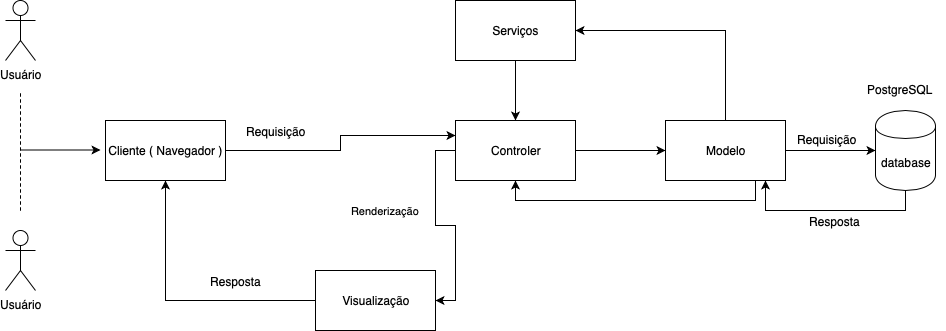
\includegraphics[width=15cm]{Monografia-FormatoLatex/Imagens/ArquiteturaEmCamadas.png}
\end{center}
}
\legend{Fonte: Criado pelo autor no site draw.io}
\label{fig:arquitetura-fluxograma}
\end{figure}

\subsection{Cliente ( Navegador )}

Toda interface que se pode visualizar os dados. Porém para a nossa aplicação utilizaremos os navegadores, mais especificamente o Chrome.

\subsection{Controller}

O controller é a parte da aplicação que intermediará o modelo e a visualização.

\subsection{Serviços}

A camada de serviço é um objeto simples Ruby que encapsula um conjunto de lógica de negócios, movida do controller ou até mesmo do modelo para ser ter configurações e regras mais focadas.

\subsection{Modelo}
A camada de modelo nos permite escrever todas as regras de negócio de uma aplicação. É também a camada que permite se comunicar com o banco de dados, executando assim os famosos CRUDs.

\subsection{Banco de dados}

A camada de modelo tem acesso ao banco de dados através da ORM. O ORM (Object Relational Mapper) é um mapeador relacional de objetos. Isso significa que você não precisa chamar manualmente o banco de dados, o ORM lida com isso para você.

\subsection{Visualização}

A camada de visualização é responsável por pegar as informações que o controller e representar essas informações. É importante informar que a camada de visualização pode representar os dados em diversos formatos, alguns: XML, CSV, JSON e HTML.

\section{Implementação da arquitetura em camadas}

Como a arquitetura em camadas tende a utilizar todas as partes do software em um único projeto, temos aqui nas pastas do Ruby on Rails pastas bem definidas para essas camadas. Caso queira ter acesso ao código fonte o mesmo está no link: https://gitlab.com/rdxinho/pibict é necessário a solicitação de acesso.


\subsection{Cliente ( Navegador )}

Como interface utilizaremos os navegadores para interagir com o sistema. O navegador faz uma requisição e recebe uma resposta e isso pode ficar mais claro utilizando o DevTools do Chrome. Na aba networking visualizamos diversas informações falaremos aqui algumas brevemente, pois não é o ponto focal do projeto. Nas figuras \ref{fig:devtools-waterfall} \ref{fig:devtools-ordem-de-arquivos} \ref{fig:devtools-status-barra}

\begin{figure}[htbp]
\hypertarget{arquitetura}{%
\caption{ Lista de todos os arquivos carregados para renderizar a página }
\begin{center}
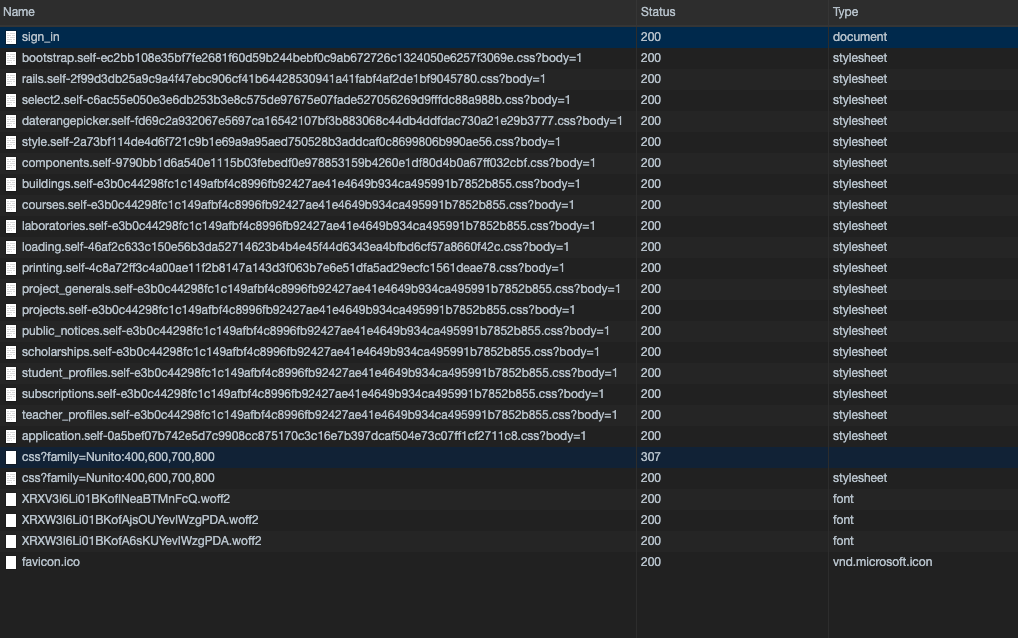
\includegraphics[width=15cm]{Monografia-FormatoLatex/Imagens/ordem-dos-arquivos-carregados.png}
\end{center}
}
\legend{Fonte: Criado pelo autor, uma imagem printada do navegador Chrome}
\label{fig:devtools-ordem-de-arquivos}
\end{figure}



\begin{figure}[htbp]
\hypertarget{arquitetura}{%
\caption{ Gráfico de carregamento dos arquivos }
\begin{center}
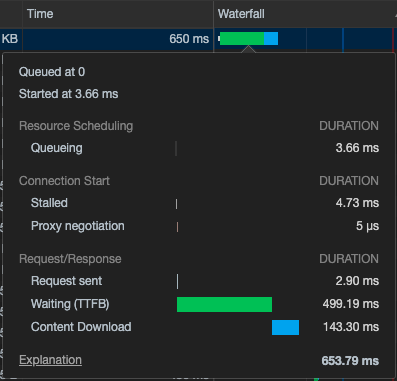
\includegraphics[width=15cm]{Monografia-FormatoLatex/Imagens/informacoes-do-waterfall.png}
\end{center}
}
\legend{Fonte: Criado pelo autor, uma imagem printada do navegador Chrome}
\label{fig:devtools-waterfall}
\end{figure}



\begin{figure}[htbp]
\hypertarget{arquitetura}{%
\caption{ Barra de status com algumas informações }
\begin{center}
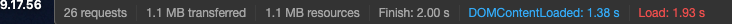
\includegraphics[width=15cm]{Monografia-FormatoLatex/Imagens/status-request-file-size.png}
\end{center}
}
\legend{Fonte: Criado pelo autor, uma imagem printada do navegador Chrome}
\label{fig:devtools-status-barra}
\end{figure}



\subsection{Controller}

O controller são responsáveis por orquestrar o modelo e a visualização. No framework Rails utilizamos uma pasta em \textbf{app/controllers} para adicionar todos os 'orquestradores' da nossa aplicação. É a responsável por receber um request e responder a um request.



\begin{figure}[htbp]
\hypertarget{arquitetura}{%
\caption{ Um código simples para ilustrar o código de um controller }
\begin{center}
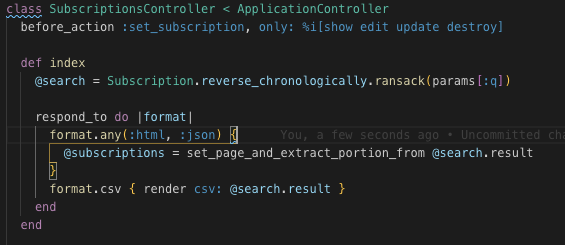
\includegraphics[width=15cm]{Monografia-FormatoLatex/Imagens/controller-camadas-exemplo.png}
\end{center}
}
\legend{Fonte: Criado pelo autor, uma imagem do código PIBICT}
\label{fig:controller-camadas}
\end{figure}


\subsection{Serviços}

Como a arquitetura baseada no modelo Model, View e Controller(MVC) enfrenta alguns problemas, adicionamos algumas camadas extras como por exemplo a camada de Serviços. Podemos criar diversos serviços com regras definidas baseada em uma determinada lógica de domínio. O controller tem uma responsabilidade muito bem definida, que é receber a requisição, verificar o que será feito, receber aquele dado e responder ao cliente. Quando ele (quem?) começa a ter lógica, já começamos a ver um espaço para a utilização de uma camada extra, que é a camada de serviço. Podemos verificar um código de serviço na figura \ref{fig:service-camadas}.


\begin{figure}[htbp]
\hypertarget{arquitetura}{%
\caption{ Um código simples para ilustrar o código de um serviço }
\begin{center}
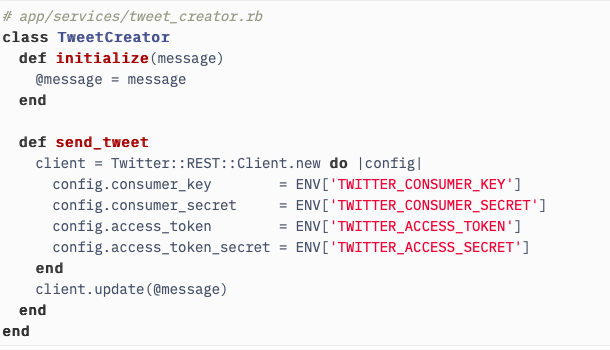
\includegraphics[width=15cm]{Monografia-FormatoLatex/Imagens/examplo-camada-service.png}
\end{center}
}
\legend{Fonte: Imagem retirada do link https://www.toptal.com/ruby-on-rails/rails-service-objects-tutorial }
\label{fig:service-camadas}
\end{figure}



\subsection{Modelo}
O Ruby on Rails também nos dá uma estrutura de pasta pronta para receber os modelos. Essa estrutura fica em \textbf{app/models}.

\begin{figure}[htbp]
\hypertarget{arquitetura}{%
\caption{ Um código simples para ilustrar o código do modelo }
\begin{center}
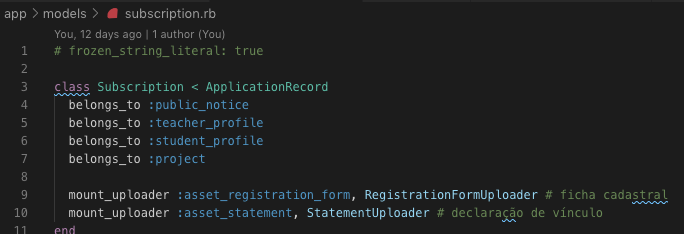
\includegraphics[width=15cm]{Monografia-FormatoLatex/Imagens/exemplo-model.png}
\end{center}
}
\legend{Fonte: Imagem retirada do link https://www.toptal.com/ruby-on-rails/rails-service-objects-tutorial }
\label{fig:service-model}
\end{figure}


\subsection{Banco de dados}

O projeto utilizará o banco de dados PostgreSQL.

\subsection{Visualização}

Os dados serão representados utilizando o HTML, CSS e Javascript. O Ruby on Rails nos dá também o ERB para dinamicamente podermos fazer essas junção dos dados retornados pelo controller.        % Implement\c{c}\~{a}o
%% TCC - Monografia
%% Ci\^{e}ncia da Computa\c{c}\~{a}o - LCMAT - CCT - UENF, 2018
%% 

\chapter{Arquitetura microsserviços}\label{cap5}

\section{Criação do fluxo das arquiteturas}

Como todo projeto a ser desenvolvido, precisamos planejar e analisar todas as tecnologias, fluxos e informações sobre o que desejamos fazer. No desenvolvimento de software não é diferente, precisamos criar um fluxograma da arquitetura.

O planejamento da arquitetura baseada em microsserviços seguirá os mesmos passos já feito para a arquitetura em camadas. O fluxograma tem uma visão macro da comunicação entre os sistemas e na fase de implementação seguiremos o fluxograma e modificaremos ao longo do processo.

\subsubsection{Fluxograma da arquitetura baseada em microsserviços}

O projeto baseado nesse tipo de arquitetura segue a utilização de diversos serviços distintos que se comunicam entre si como pode ser verificar no fluxograma da \ref{fig:microservice-fluxograma}.

O projeto para nos dará dados estatísticos sobre o assédio moral ou sexual nas Universidade, cidades, estados e países, e também será uma aplicação colaborativa, onde não sabemos a quantidade de usuários que iremos atingir e quantos desenvolvedores irão colaborar com esse projeto, então, uma arquitetura baseada em microsserviços poderá ser uma escolha ótima escolha, haja visto que poderemos contar com diversas comunidades, seja em termos de desenvolvimento de novas funcionalidades com as funcionalidades que poderão ser feitas em qualquer tecnologias e também em termos de acesso por diversos departamentos ou instâncias da sociedade, como departamento de segurança, Universidades, empresas de seguro com o intuito de analisar os riscos sobre uma determinada apólice ou mesmo a população, tendo em vista que com informações reais a cobrança será muito mais bem fundamentada para cobrar os governantes. 

\begin{figure}[htbp]
\hypertarget{arquitetura}{%
\caption{UML mostrando o fluxo da arquitetura baseada em microsserviços}
\begin{center}
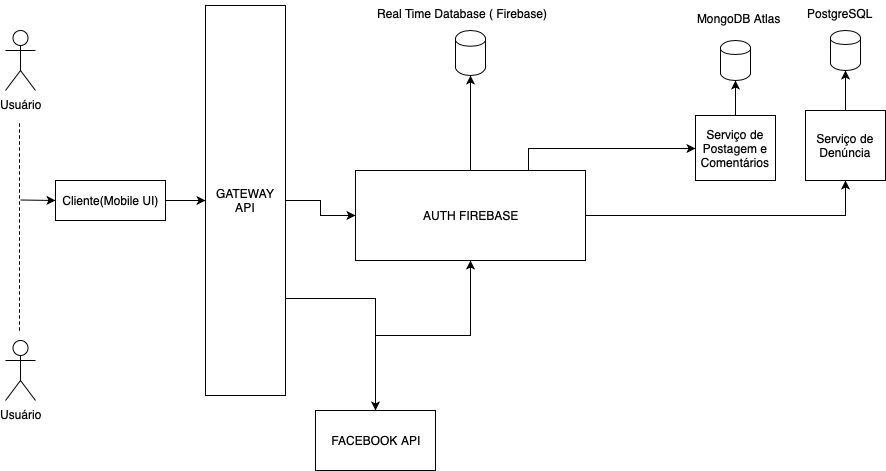
\includegraphics[width=15cm]{Monografia-FormatoLatex/Imagens/microservice-fluxograma.png}
\end{center}
}
\legend{Fonte: Criado pelo autor no site draw.io}
\label{microservice-fluxograma}
\end{figure}

\subsection{Cliente (Mobile UI)}
  
  A arquitetura proposta precisa de uma interface de entrada de dados para iteração dos usuários. O usuário executa uma ação no cliente que no nosso caso é um aplicativo mobile e inicia o fluxo que vai para a parte do API Gateway.
  
\subsection{API Gateway}

  Quando se desenvolve um sistema baseado na arquitetura de microsserviços alguns problemas aparecem, como por exemplo, precisaríamos fazer o cliente, que poderia ser um outro sistema, aplicativo, página web ou qualquer outra forma de consumir uma API conhecer diversos endpoints e versões das APIs e não seria uma forma transparente como um monolítico é, então criamos um microsserviços para cuidar dessa parte de redirecionar, verificar a autorização e a permissão do usuário. Imagino um cenário de uma arquitetura baseada em microsserviços com uns 20 sistemas, como você faria para fazer a autorização e a autenticação dos seus usuários? seria bem complexo, correto? Porém com um único ponto de entrada você torna esse processo mais simples.

\subsection{Serviço de Postagem e Comentários}

Os microsserviços são totalmente isolados e por isso cada parte tem o seu próprio banco de dados. Como podemos analisar na figura \ref{fig:microservice-fluxograma}. O serviço de postagem e comentários tem o contexto de cadastrar, excluir, deletar ou atualizar um comentário ou uma postagem. Como a postagem está totalmente acoplada aos comentários que foram feitas nele. Por exemplo, uma postagem que vamos dar o nome de \textbf{postagem1} está ligado aos comentários que vamos chamar de \textbf{comentario}, \textbf{comentario2} e \textbf{comentario}. Nesse contexto não faria sentido termos dois serviços um postagem e o outro para comentários, visto que eles fazem parte de um contexto definido.

\subsection{Serviço de Denúncia}

O serviço para denúncias também faz parte de um contexto próprio com seu banco de dados também próprio. As informações de cadastro e acompanhamento da denuncia será feita totalmente por esse serviço. O usuário poderá em um passo a passo fazer a denúncia do ocorrido e a plataforma se encarregará de enviar essas informações para um órgão competente, por exemplo nas Universidades.


\section{Implementação da Arquitetura}

O código da implementação dos microsserviços seguem abaixo:


\begin{enumerate}
    \item API Users - https://github.com/rodolfopeixoto/obsidium-users-api
    \item API Gateway - https://github.com/rodolfopeixoto/obsidium-gateway-api
    \item Interface Mobile - https://github.com/amog-oliveira/obsidium/tree/develop
    \item PostIt - https://github.com/rodolfopeixoto/obsidium-postit
\end{enumerate}

\subsection{Cliente (MOBILE UI) }

 O cliente foi desenvolvido em React Native como já informado no capítulo 2, é uma tecnologia muito utilizada para se criar aplicativos nativos com uma maior produtividade de reutilização de código para duas ou até três plataformas distintas, como por exemplo Web, IOS e Android.

\subsection{API Gateway}

A API Gateway foi desenvolvida em NodeJS com Express. A API Gateway é responsável por fazer o redirecionamento paras as rotas corretas dos microsserviços, entretanto, antes da comunicação entre ela e outros serviços, é feita uma verificação de autenticação e a autorização, onde há uma comunicação com um outro serviço especializado em usuários e autenticação e autorização de forma transparente.

\subsubsection{Serviço de usuário (Firebase e API Facebook) }

O Firebase tem um importante papel no nosso sistema, pois ele nos da um sistema de autorização e autenticação pronto e um banco de dados para armazenar essas informações. Com ele podemos verificar se usuário através de sua interface pode acessar determinado recurso ou não.

A API do Facebook tem o papel de facilitar a vida dos usuários que querem acessar o sistema rapidamente, sem perder tempo com cadastros longos ou com senhas que se perdem ao longo do tempo.

\subsection{ Serviço de Postagem e Comentários }

O serviço de postagem e comentários foi desenvolvido também em NodeJS e Express, porém o banco de dados utilizado é o banco MongoDB Atlas. O sistema utiliza um banco de dados NoSQL e remoto, pois o banco de dados Atlas é um cloud com uma interface de fácil configuração e implementação, com o banco de dados remoto, não precisamos nos preocupar com a infra-estrutura mantida. 

\subsection{ Serviço de Denúncia }

O sistema de serviço de denúncias foi desenvolvido em Ruby on Rails com PostgreSQl e ambos containerizados e hospedados no heroku. É uma API relativamente simples que cadastra as denúncias e retorna as mesmas.
        % Implement\c{c}\~{a}o

% ---
% Finaliza a parte no bookmark do PDF, para que se inicie o bookmark na raiz
% ---
\bookmarksetup{startatroot}%
% ---
% ---
%% TCC - Monografia
%% Ci\^{e}ncia da Computa\c{c}\~{a}o - LCMAT - CCT - UENF, 2018
%% 

% ---
\chapter*[Conclus\~{a}o]{Conclus\~{a}o}                  \label{conclusao}
\addcontentsline{toc}{chapter}{Conclus\~{a}o}

% As conclus\~{o}es deste trabalho podem ser divididas em tr\^{e}s partes: sobre as dificuldades encontradas no desenvolvimento do TCC, sobre o que foi feito para atingir os objetivos, e sobre o que poder\'{a} ser feito no futuro para melhorar ou complementar a pesquisa na dire\c{c}\~{a}o deste trabalho.

% Sobre as dificuldades encontradas podemos mencionar as seguintes:
% Neste trabalho foi considerado o estudo de alguns aspectos te\'{o}rico-pr\'{a}ticos da engenharia de requisitos e
% Vale a pena observar que por raz\~{o}es pr\'{a}ticas desse trabalho, no estudo de caso n\~{a}o foram consideradas todos os.....

% A metodologia utilizada, facilitou a descoberta e a classifica\c{c}\~{a}o dos mesmos, pois foi observado que quanto mais

% Em futuros trabalhos, poder\~{a}o ser considerados tamb\'{e}m, ....
%\section{Dificuldades}

Durante o desenvolvimento deste trabalho de Monografia, a maior dificuldade talvez tenha sido na escrita e no entendimento do como mostrar o problema e a hipótese que se queria trabalhar.
%\section{Objetivos}
O objetivo deste trabalho de monografia foi atingido a partir da implementação computacional das duas arquiteturas apresentadas, tendo uma experiência prática para gerar os resultados em quanto a escalabilidade, manutenibilidade e uso de multi-tecnologias que serão mostrados a seguir. 
%\section{O que poderá ser feito para melhorar ou complementar o trabalho}
Em relação a uma melhoras deste trabalho, acredita-se necessário evoluir a arquitetura e testar outras formas como por exemplo \textit{performance}, comunicação via mensagens, assim como outras abordagens da arquitetura baseada em microsserviços. %, seria muito rico para complementar o trabalho. 

%\section{Resultados Finais}
Com a experiência do desenvolvimento da arquitetura em camadas e também da baseada em microsserviços podemos listar alguns pontos sobre ambas as arquiteturas.
%\subsection{Implementação da Arquitetura}
A implementação baseada em microsserviços se mostrou bem mais complexa e demorada, haja visto que você precisa construir diversas camadas, duplica código e sua implementação exige cautela. A monolítica é muito mais simples, pois tudo que você precisa está disponível em um só lugar.

%\subsection{Escalabilidade}
Em termos de escalabilidade ambas arquiteturas se comportam bem, porém com uma arquitetura baseada em microsserviços você tem a facilidade de escalar um determinado contexto que tenha se tornado um gargalo, o que gera também diminuição de custos. Uma arquitetura monolítica, você terá a necessidade de levantar a base toda do código, muitas vezes o gargalo é em uma determinada funcionalidade e mesmo assim, teríamos que levantar toda a base de código.

%\subsection{Manutenibilidade}
Já do ponto de vista da manutenção, a arquitetura monolítica mostrou-se ser um pouco mais complexa, visto que muitas vezes se faz necessário entender algumas regras mais abrangentes. A arquitetura de microsserviços se mostrou mais simples de evoluir e manter, haja vista que são contextos menores e se há uma falha naquele contexto, vamos direto na parte que está com \textit{bug}.

%\subsection{Multi tecnologia}

Há complexidade em adicionar novas linguagens de programação ou frameworks em uma arquitetura monolítica, haja visto que esse tipo de arquitetura não foi projetada com esse intuito, porém é possível. Com a arquitetura baseada em microsserviços ficou claro que é mais fácil de se desenvolver contextos em tecnologias que favoreçam a resolução daquele contexto, pois haverá pequenos projetos com complexidades menores para se manter. Por exemplo, na abordagem criada em microsserviços, a textit{API Gateway} foi implementada para um contexto específico, ser a porta de entrada das requisições e o mesmo ser o único sistema a se comunicar com os outros sistemas internos. Para a resolução desse problema o NodeJS foi a escolha, porém poderiamos utilizar o framework Ruby on Rails. 

%\subsection{Deploy}
Já em relação ao deploy também na arquitetura baseada em microsserviço foi mais rápido, porém mais complexa, pois são diversos sistemas. A vantagem da arquitetura em camadas é que, a mesma, é enviada uma única vez; como o sistema exemplo utilizado neste trabalho ainda é pequeno o deploy mesmo sendo mais demorado que a baseada em microsserviços, ainda sim é muito rápido.

%\subsection{Logs}
Um grande problema da arquitetura baseada em microsserviços são os logs descentralizados e precisamos aqui recorrer a um software de terceiros (qual?), mais um software que demanda manutenção. Com o monolítico não é necessário, visto que os logs já estão centralizados na aplicação.
%\subsection{Autorização e Autenticação}

Em relação à autorização e autenticação, a arquitetura monolítica é mais simples e rápida a implementação, pois no exemplo deste trabalho utilizamos uma gem chamada \textit{devise} a configuramos facilmente. Já no microsserviços há todo um contexto para se preocupar, mesmo com o Firebase nos facilitando de desenvolver a parte de autenticação.

%\subsection{tolerância a falhas}
A arquitetura monolítica se for bem projetada há possibilidade de projetar uma arquitetura dessas para ser ante falhas em termos de código e de forma mais manual. Mas de modo geral, caso deixe de funcionar uma parte da aplicação, normalmente será um efeito colateral, por exemplo o banco de dados por algum motivo ter um problema, a aplicação inteira sofre esse efeito.

A arquitetura baseada em microsserviços consegue lidar muito bem com esse problema, caso não seja a parte central como a de usuário, Autenticação, autorização ou a API Gateway no caso desse projeto. Como são partes centrais, elas sofrem efeitos em cadeia e você não terá acesso ao sistema. Mas caso seja um problema na parte de comentários e posts, não teríamos problema para acessar outras partes do software, pois iria carregar normalmente em nossa aplicação mobile.

Para essa comparação podemos analisar que depende muito do que estaríamos descrevendo sobre tolerância a falhas.

%\subsection{Resumo final}
De forma geral e para concluir este trabalho, é importante entender que não há melhor arquitetura, mas sim a que mais vai se adequar a aquele projeto e equipe. Diante de tantas informações que foi possível extrair desse projeto, acredito que o melhor é obter a compreensão que as arquiteturas quando bem estudadas e aplicadas de forma correta poderá diminuir e aumentar a produtividade da equipe em resolver problemas.


\section{Trabalhos Futuros}
Está faltando trabalhos futuros, ou tarefas ou testes que vc considere sejam importantes de serem realizados como continuação de seu trabalho.



% Há algumas vantagens quanto ao desenvolvimento, como toda base de código está disponível em um lugar só, basta executar baixar de um repositório git sua base de código e então terá todo seu projeto disponível e de fácil acesso. Como o projeto é único a base de logs também é única, o que representa uma grande vantagem, não necessitando de um software de de terceiros. 


% Há também desvantagens, em termos de manutenção como a base de código utilizada como exemplo, na base há diversas regras de negócio e possível e ocorreu durante o desenvolvimento alguns bugs que demoraram a ser resolvido, devido a base de código e a falta de teste inicialmente. Para escalar a aplicação se faz necessário replicar toda a base de código novamente, o que aumenta o custo dos recursos.
   % Conclus\~{a}o

% ----------------------------------------------------------
% ELEMENTOS P\'{O}S-TEXTUAIS
% ----------------------------------------------------------
\postextual


% ----------------------------------------------------------
% Refer\^{e}ncias bibliogr\'{a}ficas:   \cite{abc}   \citeonline{xyz}
% ----------------------------------------------------------
%\bibliographystyle{alpha}  %%%% Outros estilos: plain, apacite, plainnat, etc.

\bibliography{minhaMonografiaBib}


% ----------------------------------------------------------
% Ap\^{e}ndices
% ----------------------------------------------------------

% ---
% Inicia os ap\^{e}ndices
% ---
\begin{apendicesenv}

% Imprime uma p\'{a}gina indicando o in\'{\i}cio dos ap\^{e}ndices
\partapendices

% ----------------------------------------------------------

% %% Prof. Ausberto S. castro Vera
% %% UENF-CCT-LCMAT -Ci\^{e}ncia da Computa\c{c}\~{a}o
% %% Adaptado de: http://www.udcsummary.info
% %% 24 de Agosto de 2018 


% \chapter{UDC - Universal Decimal Classification}  %% comentar isto para artigo

% \section{Universal Decimal Classification}

% \subsection{ O que \'{e} UDC?}

% A UDC \'{e} o principal esquema de classifica\c{c}\~{a}o multil\'{\i}ngue do mundo para todas as \'{a}reas do conhecimento e uma ferramenta sofisticada de indexa\c{c}\~{a}o e recupera\c{c}\~{a}o. \'{E} um sistema de classifica\c{c}\~{a}o altamente flex\'{\i}vel para todos os tipos de informa\c{c}\~{a}o em qualquer meio.

% Por causa de seu arranjo hier\'{a}rquico l\'{o}gico e natureza anal\'{\i}tica-sint\'{e}tica, \'{e} adequado para organiza\c{c}\~{a}o f\'{\i}sica de cole\c{c}\~{o}es, bem como para navega\c{c}\~{a}o e pesquisa de documentos. A UDC est\'{a} estruturada de tal forma que novos desenvolvimentos e novos campos de conhecimento podem ser prontamente incorporados. O c\'{o}digo em si \'{e} independente de qualquer idioma ou script em particular (consistindo de numerais ar\'{a}bicos e sinais de pontua\c{c}\~{a}o comuns) e as descri\c{c}\~{o}es de classes que o acompanham apareceram em muitas vers\~{o}es traduzidas.

% \subsection{ Quem utiliza UDC?}
% O esquema \'{e} de uso mundial e foi publicado no todo ou em parte em mais de 40 idiomas diferentes. \'{E} utilizado em servi\c{c}os bibliogr\'{a}ficos, centros de documenta\c{c}\~{a}o e bibliotecas em cerca de 130 pa\'{\i}ses em todo o mundo. Cole\c{c}\~{o}es de biblioteca indexadas por UDC podem ser encontradas em OPACs e bancos de dados da biblioteca.


% \subsection{0. SCIENCE AND KNOWLEDGE. ORGANIZATION. COMPUTER SCIENCE. INFORMATION. DOCUMENTATION. LIBRARIANSHIP. INSTITUTIONS. PUBLICATIONS}

% Tabelas Principais:

% 00 Prolegomena. Fundamentals of knowledge and culture. Propaedeutics

% 001 Science and knowledge in general. Organization of intellectual work

% 002 Documentation. Books. Writings. Authorship

% 003 Writing systems and scripts

% \textbf{004 Computer science and technology. Computing. Data processing}
% \begin{itemize}
%   \item \textbf{004.01/.08 Special auxiliary subdivision for computing}
%   \begin{itemize}
%     \item    004.01 Documentation
%     \item    004.02 Problem-solving methods
%     \item    004.03 System types and characteristics
%     \item    004.04 Processing orientation
%     \item    004.05 System and software quality
%     \item    004.07 Memory characteristics
%     \item    004.08 Input, output and storage media
%   \end{itemize}

%   \item \textbf{004.2 Computer architecture}
%   \begin{itemize}
%     \item 004.22  Data representation
%     \item     004.23 Instruction set architecture
%     \item     004.25 Memory system
%     \item     004.27 Advanced architectures. Non-Von Neumann architectures
%   \end{itemize}

%   \item \textbf{004.3 Computer hardware}
%     \begin{itemize}
%     \item004.3`1/`2 Special auxiliary subdivision for hardware
%     \begin{itemize}
%       \item 004.3`1   Production of computers
%       \item 004.3`2  Computer installations
%     \end{itemize}
%     \item 004.31  Processing units. Processing circuits
%     \item 004.32  Computer pathways
%     \item 004.33  Memory units. Storage units
%     \item 004.35  Peripherals. Input-output units
%     \item 004.38  Computers. Kinds of computer
%   \end{itemize}

%   \item \textbf{004.4 Software}
%     \begin{itemize}
%     \item 004.4`2/`6 Special auxiliary subdivision for software
%     \begin{itemize}
%       \item 004.4`2 Software development tools
%       \item 004.4`4 Programming language translation
%       \item 004.4`6 Runtime environment
%     \end{itemize}
%     \item 004.41 Software engineering
%     \item 004.42 Computer programming. Computer programs
%     \item 004.43 Computer languages
%     \item 004.45 System software
%     \item 004.49 Computer infections
%   \end{itemize}

%   \item \textbf{004.5 Human-computer interaction. Man-machine interface. User interface. User environment}
%         \begin{itemize}
%         \item 004.51 Display interface
%         \item 004.52  Sound interface
%         \item 004.55  Hypermedia. Hypertext
%         \item 004.58  User help
%         \end{itemize}

%   \item \textbf{004.6 Data}
%     \begin{itemize}
%     \item 004.62  Data handling
%     \item 004.63  Files
%     \item 004.65  Databases and their structures
%     \item 004.67  Systems for numeric data
%     \end{itemize}

%   \item \textbf{004.7 Computer communication. Computer networks}
%     \begin{itemize}
%     \item 004.71 Computer communication hardware
%     \item     004.72  Network architecture
%     \item     004.73  Networks according to area covered
%     \begin{itemize}
%       \item 004.738  Network interconnection. Internetworking
%     \end{itemize}
%     \item     004.75  Distributed processing systems
%     \item     004.77  General networking applications and services
%     \item     004.78  Online computing systems for specific use
%   \end{itemize}

%   \item \textbf{004.8 Artificial intelligence}

%   \item \textbf{004.9 Application-oriented computer-based techniques}
%     \begin{itemize}
%     \item 004.91   Document processing and production
%     \item 004.92  Computer graphics
%     \item 004.93  Pattern information processing
%     \item 004.94  Simulation
%   \end{itemize}


% \end{itemize}

% 005 Management

% 006 Standardization of products, operations, weights, measures and time

% 007 Activity and organizing. Communication and control theory generally (cybernetics). 'Human engineering'

% 008 Civilization. Culture. Progress


%% TCC - Monografia
%% Ci\^{e}ncia da Computa\c{c}\~{a}o - LCMAT - CCT - UENF, 2018
%% 24/08/2018







% ----------------------------------------------------------
\chapter{Areas de Conhecimento CNPq}
% ----------------------------------------------------------

Tabela Completa em :\\
 \url{http://www.cnpq.br/documents/10157/186158/TabeladeAreasdoConhecimento.pdf}

\begin{tabular}{ll}
  \hline
  % after \\: \hline or \cline{col1-col2} \cline{col3-col4} ...
 \textbf{ C\'{o}digo} & \textbf{\'{A}rea de Conhecimento} \\
    \hline     \hline
  10000003 & CI\^{E}NCIAS EXATAS E DA TERRA \\
    \hline
  \textbf{1.03.00.00-7}	& \textbf{Ci\^{e}ncia da Computa\c{c}\~{a}o} \\
      \hline
1.03.01.00-3	& \textit{Teoria da Computa\c{c}\~{a}o}\\
    \hline
1.03.01.01-1	& 	Computabilidade e Modelos de Computa\c{c}\~{a}o\\
1.03.01.02-0	& 	Linguagem Formais e Automatos\\
1.03.01.03-8	& 	An\'{a}lise de Algoritmos e Complexidade de Computa\c{c}\~{a}o\\
1.03.01.04-6	& 	L\'{o}gicas e Sem\^{a}ntica de Programas\\
    \hline
1.03.02.00-0	& 	\textit{Matem\'{a}tica da Computa\c{c}\~{a}o}\\
    \hline
1.03.02.01-8	& 	Matem\'{a}tica Simb\'{o}lica\\
1.03.02.02-6	& 	Modelos Anal\'{\i}ticos e de Simula\c{c}\~{a}o\\
    \hline
1.03.03.00-6	& 	\textit{Metodologia e T\'{e}cnicas da Computa\c{c}\~{a}o}\\
    \hline
1.03.03.01-4	& 	Linguagens de Programa\c{c}\~{a}o\\
1.03.03.02-2	& 	Engenharia de Software\\
1.03.03.03-0	& 	Banco de Dados\\
1.03.03.04-9	& 	Sistemas de Informa\c{c}\~{a}o\\
1.03.03.05-7	& 	Processamento Gr\'{a}fico (Graphics)\\
    \hline
1.03.04.00-2	& 	\textit{Sistemas de Computa\c{c}\~{a}o}\\
    \hline
1.03.04.01-0	& 	Hardware\\
1.03.04.02-9	& 	Arquitetura de Sistemas de Computa\c{c}\~{a}o\\
1.03.04.03-7	&	Software B\'{a}sico\\
1.03.04.04-5	&	Teleinform\'{a}tica\\
  \hline
\end{tabular}

% ----------------------------------------------------------

\end{apendicesenv}
% ---


\end{document}







% ----------------------------------------------------------
% Gloss\'{a}rio
% ----------------------------------------------------------
%
% Consulte o manual da classe abntex2 para orienta\c{c}\~{o}es sobre o gloss\'{a}rio.
%
%\glossary

% ----------------------------------------------------------
% Ap\^{e}ndices
% ----------------------------------------------------------
% ---
% Inicia os ap\^{e}ndices
% ---
\begin{apendicesenv}

% Imprime uma p\'{a}gina indicando o in\'{\i}cio dos ap\^{e}ndices
\partapendices

% ----------------------------------------------------------
\chapter{Quisque libero justo}
% ----------------------------------------------------------

\lipsum[50]

% ----------------------------------------------------------
\chapter{Nullam elementum urna vel imperdiet sodales elit ipsum pharetra ligula
ac pretium ante justo a nulla curabitur tristique arcu eu metus}
% ----------------------------------------------------------
\lipsum[55-57]

\end{apendicesenv}
% ---


% ----------------------------------------------------------
% Anexos
% ----------------------------------------------------------

% ---
% Inicia os anexos
% ---
\begin{anexosenv}

% Imprime uma p\'{a}gina indicando o in\'{\i}cio dos anexos
\partanexos

% ---
\chapter{Morbi ultrices rutrum lorem.}
% ---
\lipsum[30]

% ---
\chapter{Cras non urna sed feugiat cum sociis natoque penatibus et magnis dis
parturient montes nascetur ridiculus mus}
% ---

\lipsum[31]

% ---
\chapter{Fusce facilisis lacinia dui}
% ---

\lipsum[32]

\end{anexosenv}

%---------------------------------------------------------------------
% INDICE REMISSIVO
%---------------------------------------------------------------------

\printindex

\end{document}
